


\section{Introduction}
\label{sec:banffintroduction}

In this section, the \Gls{ND} inclusive electron (anti-) neutrino
samples and the \Gls{ND} muon (anti-) neutrino samples in \Gls{RHC}
are used in the context of oscillation analysis. This was never
realised previously on \Gls{TK}. This study has three goals, two of
which are related to the electron (anti-) neutrino appearance samples
at \Gls{SK} in light of the search for \Gls{CP} violation in the
neutrino sector. The other goal is related to the muon (anti-)
neutrino disappearance measurement at \Gls{TK}. These goals are:
\begin{itemize}[noitemsep,topsep=0pt]
\item The consolidation of the result for \Gls{CP} violation by moving
  from a theory-driven electron neutrinos cross section uncertainty to
  an equivalent data-driven uncertainty.
\item An overall the reduction of systematic uncertainties related to
  the electron (anti-) neutrinos appearance samples at \Gls{SK}: as
  will be shown in this chapter, the data result can be improved
  simply by collecting more data, as opposed to the theory-driven
  error.
\item Finally, this study can be used for testing the single pion
  model in the anti-neutrino sector. This has some importance in the
  oscillation in the atmospheric sector using the anti-neutrino
  disappearance samples.
\end{itemize}

In the second section, the oscillation analysis strategy is
explained. Then, the framework for characterising the oscillation
analyses systematic uncertainties with the \Gls{ND} is described, and
the samples used in the fit are described. In the subsequent sections,
the expected sensitivity and the data result are shown. Finally, the
propagation of the sensitivity to the \Gls{CP} violation allowed
region is shown.


\section{The TK oscillation analysis strategy}
\label{sec:oscillationanalysis}
In this section, the strategy for the oscillation analyses in \Gls{TK}
is explained. There are three main analyses on \Gls{TK} that produce
the oscillation parameter results. Two of them use a semi-frequentist
approach and aim to produce confidence intervals on oscillation
parameters, and run a fit over them and the nuisance parameters.
These two analyses are called ``\gls{p-theta}'' and
``\Gls{VALOR}''~\cite{VALOR}, both of them use a
Minuit2~\cite{James:1975dr} log-likelihood fit. The other one uses a
Markov-Chain Monte Carlo (\Gls{MCMC}) to sample over the parameter
space; it is called ``\Gls{MaCh3}''~\cite{MACH3}. It is a fully
Bayesian analysis and produces credible intervals on neutrino mixing
parameters.

The fact that the oscillation analyses are repeated by different
groups allows validation and comparisons of the result.

These analyses use the multiple inputs from different \Gls{TK}
groups. The inputs are listed here:
\begin{itemize}
\item The beam group provides the absolute flux histograms (such as
  the one shown in Figure~\ref{fig:flux1}), the flux covariance matrix
  which encloses all the systematic errors on these histograms (see
  Figure~\ref{fig:flux2} and Section~\ref{sec:fluxsyst}) and the flux
  tuning which is, as described in Section~\ref{fig:beamline},
  determined from {\it in situ} measurements of the beam and
  additional hadron production data from
  NA61~/~SHINE~\cite{Abgrall:2011ae,Abgrall:2011ts,Abgrall:2015hmv}.
\item The neutrino interaction working group (\Gls{NIWG}) provides a
  parametrisation for the cross section and ``prefit'' systematic
  errors on each of the nuisance parameter of interest. These
  generally rely on the use of external data sets and fit such as the
  one described in~\cite{CallumFit}, discussions with theorists, and
  phenomenology work done within \Gls{TK}.
\item The \Gls{ND} data, which is used before the main oscillation fit
  to constrain the flux and cross section systematic
  uncertainties. Traditionally, the \Gls{ND} data that was used for
  the fits was restricted to the \Gls{numu} and \Gls{anumu} data,
  however the aim of this analysis is to include samples sensitive to
  the background \Gls{nue} flux (which represent around $1\%$ of the
  neutrino at the flux peak) to constrain cross section and flux
  parameters. Fitting these parameters with such samples can introduce
  anti-correlation between flux and cross section parameters (i.e. at
  constant number of \Gls{nue} in the \Gls{ND}, if the flux increases,
  the cross section has to decrease).
\item The \Gls{SK} \Gls{CCQE}-like \gls{numu}, \gls{nue}, \gls{anumu}
  and \gls{anumu} samples, and the \Gls{nue} \Gls{CC}$1\pi^+$ sample.
\end{itemize}

Note that the statistical power of the data from the \Gls{ND} is much
larger than the one from \Gls{SK}. This means that \Gls{ND} data
uncertainty is largely dominated by systematic uncertainties, whereas
the \Gls{SK} data uncertainty is mostly statistical (especially for
the appearance samples, the \gls{nue} and \gls{anue} samples),
although this is becoming less and less true as \Gls{TK} data is being
collected.

For all the three oscillation analyses, the first step is to fit the
\Gls{ND} data to constrain flux and cross section parameters. Once an
acceptable fit ($p_\text{value} > 5\%$) is reached, it is considered
that the parametrisation is sufficient for an oscillation fit and the
errors are propagated to \Gls{SK}.

There are other mechanisms to check that the parametrisation is
sufficient under significant change of cross section model, called
fake data, but these are beyond the scope of the analysis that is
presented here.

In this section, the focus is on the \Gls{ND} fits that are used in
oscillation analyses. This step is essential to reduce the systematic
uncertainties on the cross section and neutrino flux.


\section{Beam and Near Detector Fit Framework}
\label{sec:BANFF}
The software framework used for this is called \Gls{BANFF}. It
performs a Minuit2~\cite{James:1975dr} fit and minimises the Poisson
logarithmic likelihood with extra $\chi^2$ penalty terms for the
systematic error. They are defined as follows:

\begin{align}
  \label{eq:likelihood}
  -2\ln(\mathcal{L}) &= 2 \sum_{i=0}^{\text{N bins}}N^{p}_{i}(\vec{b},\vec{x},\vec{d})-N^{d}_{i}
                       +N^{d}_{i}\ln[N^{d}_{i}/N^{p}_{i}(\vec{b},\vec{x},\vec{d})] \\
                     &+\sum_{k,l=0}^{E_{\nu}\text{~bins}}\Delta b_{k}(V^{-1}_\text{beam})_{k,l}\Delta b_{l} \nonumber \\
                     &+\sum_{m,n=0}^{\text{xsec param}}\Delta x_{m}(V^{-1}_\text{xsec})_{m,n}\Delta x_{n} \nonumber \\
                     &+\sum_{i,j=0}^{\text{N bins}}\Delta d_{i}(V^{-1}_{\text{det}})_{i,j}\Delta d_{j},\nonumber 
\end{align}
where $\mathcal{L}$ is the total likelihood (note that
$-2\ln(\mathcal{L})$ can be approximated to a $\chi^2$ function for
sufficient statistics), $i$ and $j$ are the bin numbers for the
reconstructed quantities $p_\text{lepton}$ (momentum of the leading
lepton) and $\cos(\theta_\text{lepton})$ (cosine of the angle between
the neutrino direction and the leading
lepton). $N^{p}_{i}(\vec{b},\vec{x},\vec{d})$ is the number of
expected events in the $i^{\text{th}}$ bin, which depends on
$\vec{b}$, the beam weight, which encloses the action of the flux
systematic uncertainties on the events; $\vec{x}$, the cross section
weight, which parametrises the effect of the cross section systematic
uncertainties and $\vec{d}$, the detector weight, which parametrises
the detector uncertainty in each reconstructed bin. $N^d_i$ is the
number of events seen in the $i^{\text{th}}$ bin.

$V_\text{beam}$, $V_\text{xsec}$ and $V_\text{det}$ represent the
covariance matrices of the flux, cross section and detector systematic
uncertainties, respectively. They respectively correlate: the number
of neutrinos in each true energy bin in the case of the flux, the
cross section parameters, and the number of events in each
reconstructed bin. $\Delta b$, $\Delta x$, $\Delta d$, are the
variations of the beam, cross section and detector parameters with
respect to their nominal values, respectively.

\section{Samples used}
\label{sec:samples}
The samples that are used are \Gls{ND} ``tracker'' samples (i.e. they
do not include the analyses where the \Gls{PD} is used as a
target). These analyses are divided according to their topology,
detector (\Gls{FGD} 1 or 2) and whether the neutrino beam is running
in neutrino mode (\Gls{FHC}) or anti-neutrino mode
(\Gls{RHC}). Twenty-eight binned samples are used in the fit. The
first six samples have not changed compared to previous analyses:
\begin{itemize}[noitemsep,topsep=0pt]
\item 3 \Gls{numu} \Gls{CC} selections in \Gls{FGD}1 in \Gls{FHC}: 1
  muon + 0 pion; 1 muon + 1 positively charged pion; 1 muon +
  everything else;
\item 3 \Gls{numu} \Gls{CC} selections in \Gls{FGD}2 in \Gls{FHC}: 1
  muon + 0 pion; 1 muon + 1 positively charged pion; 1 muon +
  everything else.
\end{itemize}
The remaining samples are new selections that have been used for the
first time in this fit:
\begin{itemize}[noitemsep,topsep=0pt]
\item 3 \Gls{anumu} \Gls{CC} selections in \Gls{FGD}1 in \Gls{RHC}: 1
  anti-muon + 0 pion; 1 anti-muon + 1 negatively charged pion; 1
  anti-muon + everything else;
\item 3 \Gls{anumu} \Gls{CC} selections in \Gls{FGD}2 in \Gls{RHC}: 1
  anti-muon + 0 pion; 1 anti-muon + 1 negatively charged pion; 1
  anti-muon + everything else;
\item 3 \Gls{numu} \Gls{CC} selections in \Gls{FGD}1 in \Gls{RHC}: 1
  muon + 0 pion; 1 muon + 1 positively charged pion; 1 muon +
  everything else;
\item 3 \Gls{numu} \Gls{CC} selections in \Gls{FGD}2 in \Gls{RHC}: 1
  muon + 0 pion; 1 muon + 1 positively charged pion; 1 muon +
  everything else;
\item Inclusive \Gls{nue} \Gls{CC} selection in \Gls{FGD}1 in
  \Gls{FHC};
\item Inclusive \Gls{nue} \Gls{CC} selection in \Gls{FGD}2 in
  \Gls{FHC};
\item Inclusive \Gls{anue} \Gls{CC} selection in \Gls{FGD}1 in
  \Gls{RHC};
\item Inclusive \Gls{anue} \Gls{CC} selection in \Gls{FGD}2 in
  \Gls{RHC};
\item Inclusive \Gls{nue} \Gls{CC} selection in \Gls{FGD}1 in
  \Gls{RHC};
\item Inclusive \Gls{nue} \Gls{CC} selection in \Gls{FGD}2 in
  \Gls{RHC};
\item Photon sample in \Gls{FGD}1 selection in \Gls{FHC};
\item Photon sample in \Gls{FGD}2 selection in \Gls{FHC};
\item Photon sample in \Gls{FGD}1 selection in \Gls{RHC};
\item Photon sample in \Gls{FGD}2 selection in \Gls{RHC}.
\end{itemize}

For previous iterations of these fits~\cite{TN324}, the \Gls{RHC} were
using a different categorisation, and had a split between \Gls{numu}
\Gls{CC} with one or several tracks (so-called ``\Gls{CC} 1-track''
and ``\Gls{CC} n-tracks''). The electron samples had never been used
in the these fits. However, they are used in \Gls{NOvA}
analyses~\cite{PhysRevLett.118.231801}).

The remainder of this section covers the description of the samples
used and how they are selected. Firstly, the amount of \Gls{POT} that
is used is shown. Then, the selections are broadly described. The
binning used is detailed in Appendix~\ref{app:binning}.

\subsection{Run periods and Proton On Target}
\label{subsec:pot}
The data sets used correspond to the data collected with the \Gls{ND}
when all the sub-detectors are in place (excluding run~1), up to
summer 2017, all the corresponding \Gls{POT} is listed in
Table~\ref{tab:POTBANFF}. Note that the year 2017 data was only
partially calibrated (so called ``\gls{pc1}''), which is different
from all the rest of the data which was fully calibrated
(``\gls{rdp},'' for real data processing). The \Gls{ECal} run~8 data
was not fully calibrated at the time this document was written. This
has an impact on the \Gls{nue} selections which are using the
\Gls{ECal} for \Gls{PID}, as will be explained in the next section, so
the run~8 data was not used for the electron neutrino
selections. However, this has no impact on the muon neutrinos
selections, so this data was used for these selections.

\begin{table}[ht]
  \begin{adjustbox}{center}
    \begin{tabular}{llllll}
      \toprule
      \multirow{2}{*}{Runs} & \multicolumn{5}{c}{POT}\\
                            & Data & \multicolumn{2}{l}{\Gls{magnet} \Gls{MC} (ratio)} & \multicolumn{2}{l}{\Gls{sand} \Gls{MC} (ratio)} \\
      \midrule
      2a  (\Gls{FHC}) & $3.59\times 10^{19}$ & $9.24\times 10^{20}$&$(0.0389)$ & $3.71\times 10^{19}$&$(0.968)$ \\
      2w  (\Gls{FHC}) & $4.34\times 10^{19}$ & $1.2 \times 10^{21}$&$(0.036) $ & $4   \times 10^{19}$&$(1.08) $ \\
      3ba (\Gls{FHC}) & $2.17\times 10^{19}$ & $4.45\times 10^{20}$&$(0.0488)$ & $2.35\times 10^{19}$&$(0.923)$ \\
      3ca (\Gls{FHC}) & $1.36\times 10^{20}$ & $2.63\times 10^{21}$&$(0.0519)$ & $1.31\times 10^{20}$&$(1.04) $ \\
      4a  (\Gls{FHC}) & $1.78\times 10^{20}$ & $3.5 \times 10^{21}$&$(0.0509)$ & $1.74\times 10^{20}$&$(1.02) $ \\
      4w  (\Gls{FHC}) & $1.64\times 10^{20}$ & $1.89\times 10^{21}$&$(0.0868)$ & $1.6 \times 10^{20}$&$(1.03) $ \\
      5w  (\Gls{RHC}) & $4.35\times 10^{19}$ & $2.3 \times 10^{21}$&$(0.0189)$ & $9.07\times 10^{19}$&$(0.479)$ \\
      6ba (\Gls{RHC}) & $1.27\times 10^{20}$ & $1.42\times 10^{21}$&$(0.0898)$ & $3.42\times 10^{20}$&$(0.373)$ \\
      6ca (\Gls{RHC}) & $5.08\times 10^{19}$ & $5.28\times 10^{20}$&$(0.0963)$ & $1.05\times 10^{20}$&$(0.485)$ \\
      6da (\Gls{RHC}) & $7.75\times 10^{19}$ & $6.88\times 10^{20}$&$(0.113) $ & $1.58\times 10^{20}$&$(0.491)$ \\
      6ea (\Gls{RHC}) & $8.51\times 10^{19}$ & $8.59\times 10^{20}$&$(0.0991)$ & $1.75\times 10^{20}$&$(0.485)$ \\
      7w  (\Gls{RHC}) & $2.44\times 10^{20}$ & $3.37\times 10^{21}$&$(0.0723)$ & $5.04\times 10^{20}$&$(0.484)$ \\
      8a  (\Gls{FHC}) & $4.15\times 10^{20}$ & $3.63\times 10^{21}$&$(0.114) $ & $4.04\times 10^{20}$&$(1.03) $ \\
      8w  (\Gls{FHC}) & $1.58\times 10^{20}$ & $2.64\times 10^{21}$&$(0.0598)$ & $1.61\times 10^{20}$&$(0.98) $ \\
      \midrule
      Total \Gls{FHC} & $1.15\times 10^{21}$ & $1.69\times 10^{22}$&$(0.0684)$ & $1.13\times 10^{21}$&$(1.02) $ \\ 
      Total \Gls{RHC} & $6.7 \times 10^{20}$ & $9.16\times 10^{21}$&$(0.0732)$ & $1.37\times 10^{21}$&$(0.487)$ \\ 
      \bottomrule
    \end{tabular}
  \end{adjustbox}
  \caption[POT and POT ratios (data~/~MC) used for the 2018 BANFF
  analysis]{\Gls{POT} and \Gls{POT} ratios (data~/~\Gls{MC}) used for
    the \Gls{BANFF} 2018 analysis, note that the run~8 data is only
    partially calibrated (\gls{pc1}).}
  \label{tab:POTBANFF}
\end{table}

\subsection{Muon (anti-) neutrino  description}
\label{subsec:muonneutrinoselection}
All the muon selections rely on the identification of a muon starting
in the \Gls{FGD}1 or 2. Based on the topology of the remaining
particles, the event is then tagged as ``\Gls{CC} 0 pion,'' ``\Gls{CC}
1 pion'' or ``\Gls{CC} other,'' depending upon the presence of a
detected pion in the selection. Note that, other than the
reconstructed charge of the particle, the selections are identical in
\Gls{FHC} and \Gls{RHC} and for the anti-neutrino equivalent.
\begin{itemize}[noitemsep,topsep=0pt]
\item The ``\Gls{CC} 0 pion'' selections mostly contain \Gls{CCQE}
  events, but can also have some events where a pion was created
  inside the nucleus (such as resonant events) and was absorbed by the
  nucleus through \Gls{FSI}.
\item The ``\Gls{CC} 1 pion'' selections contain events where a
  positive pion was tagged, in general, this selection is dominated by
  \Gls{RES} and \Gls{COH} events, but some \Gls{CCQE} events can enter
  if the ejected proton from the interaction creates a pion through
  \Gls{FSI}.
\item The ``\Gls{CC} other'' selections are all the remaining events,
  which are mostly \Gls{DIS} and \Gls{SIS} events. All the wrong sign
  \Gls{TPC} pions can also be present.
\end{itemize}

The event selection and cuts are illustrated in
Figure~\ref{fig:flowchart}. Each cut is quickly detailed. For a more
complete description, see~\cite{TN152,TN212}.

\begin{figure}[ht]
  \center
  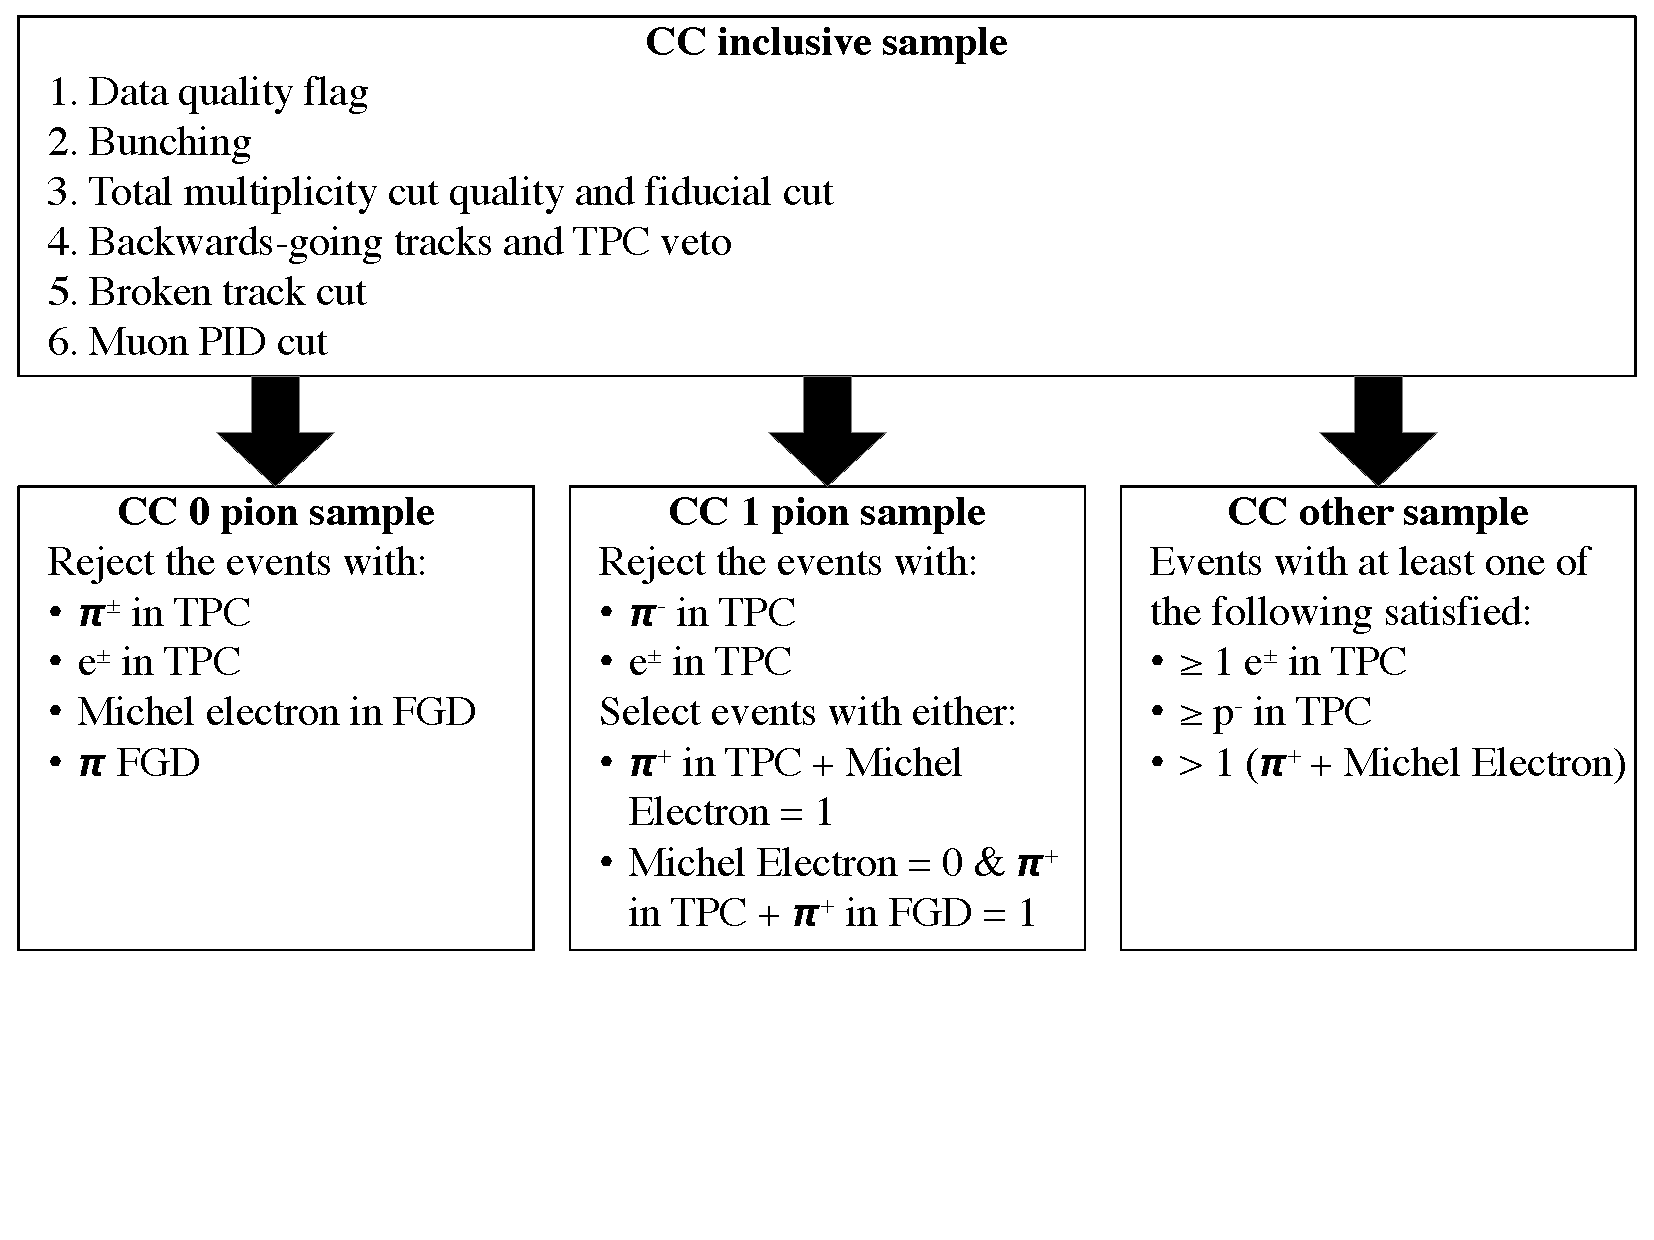
\includegraphics[width=0.8\textwidth]{images/BANFF/FlowCharSelection.pdf} \\
  \caption[The flow chart for the $\nu_\mu$ CC multi-pion
  selections]{The flow chart for the \Gls{numu} \Gls{CC} multi-pion
    selections, from~\cite{TN152}.}
  \label{fig:flowchart}
\end{figure}


\subsubsection{Data quality flag and Bunching}
These cuts are identical to the ones given in the description in
Section~\ref{sec:cutflow}.

\subsubsection{Total multiplicity cut quality and fiducial cut}
These cuts are the same as the ``Cut 1'' and ``Cut 2'' in
Section~\ref{subsec:photonselection}

\subsubsection{Backwards-going tracks and TPC veto}
It happens that tracks starting from the upstream layers of the
\Gls{FGD}1 are reconstructed as backward going tracks, especially if
the muon undergoes a hard scatter in the \Gls{FGD}1 and is
reconstructed as two tracks. To overcome this problem, an upstream
\Gls{TPC} veto was designed and if a track starts at less than
$150$~mm upstream from the main muon track, it is
rejected. Additionally, for \Gls{FGD}2 selections, if the track starts
or ends in the \Gls{FGD}1, the event is rejected.

\subsubsection{Broken track cut}
This cut was made to remove events where the reconstruction failed and,
rather than a single muon reconstructed, a short track is
reconstructed in the \Gls{FGD} and another one is reconstructed in the
last layers of the \Gls{FGD} and \Gls{TPC}. The cut therefore removes
events where a track starts in the last two layers of the \Gls{FGD} in
the downstream direction and has another isolated \Gls{FGD} track.

\subsubsection{Muon Particle Identification}
The \Gls{PID} relies on the \Gls{TPC}. If the reconstructed momentum
is smaller than $500$~MeV, then the track has to satisfy the relation:

\begin{equation}
  L_{MIP} = \frac{L_{\mu} + L_{\pi}}{1-L_p} >0.8.
\end{equation}

Then, to remove proton and pions, all the tracks have to satisfy:
\begin{equation}
  L_{\mu} > 0.05
\end{equation}

In the above equations, $L$ is the likelihood related to the \Gls{PID}
of the particle $i$ by the following equation:

\begin{equation}
  L_i = \frac{e^{-\pi_{i,\text{PID}}^2}}{\sum_l e^{-\pi_{l,\text{PID}}^2}},
  \label{eq:tpcpidlike}
\end{equation}

where $\pi_{l,\text{PID}}$ is defined in Equation~(\ref{eq:tpcpull})
and based on the difference between the expected and the measured
$dE/dx$ of the particle. The index $l$ runs over the particles:
proton, electron, muon and pion.

\subsubsection{Pion tag}
All the remaining tracks in the events are checked to create a pion
tag. They are required to start in the same \Gls{FGD} and bunch. If
the track has more than $18$ \Gls{TPC} hit\footnote{i.e. the particle
  has triggered at least $18$ MicroMegas.} and has a positive charge,
a \Gls{TPC} \Gls{PID} is realised as such:

\begin{align*}
  L_{MIP} &= \frac{L_{\mu}+L_{\pi}}{1-L_p} > 0.8 \text{~if~} p < 500 \text{~MeV/c}\\
  L_{\pi} &> 0.3 \text{~for all the tracks.} 
\end{align*}

If a track satisfies this requirement, it is tagged as a \Gls{TPC}
pion. The same quantities can be constructed for electron, positron,
proton and pion. The events containing \Gls{TPC} tracks are sorted as
indicated in the Figure~\ref{fig:flowchart}.

For a track to be tagged as a ``Michel electron'' (which, within
\Gls{TK}, means a decay electron from a charged pion or charged muon),
the requirement is to have a deposition of at least $200$
photo-electrons in the \Gls{FGD}, after the end of bunch timing
window.

Finally, the \Gls{FGD} \Gls{PID} can be realised on short pion tracks.
In that case, the track must be fully contained in the \Gls{FGD} and,
using a similar definition of the pull, as in
Equation~(\ref{eq:tpcpull}), based on the $dE/dx$ of the particle and
the energy deposited in the \Gls{FGD}, one can make a cut on its value
(in this case, $-2<\pi_{\pi \text{FGD PID}} < 2.5$).

\subsection{Electron (anti-) neutrino selections}
\label{subsec:electronneutrinoselections}
The electron (anti-) neutrino selections are now described. The
selections are aimed to select all electron (anti-) neutrino samples
and do not depend on the presence of charged pions or additional
tracks in the event. For more details on the selections, the reader
can refer to~\cite{TN282}. Future development of the selections will
probably involve the usage of more advanced event categorisation
techniques, and machine learning.  However this is still in
development within the \Gls{TK} collaboration as this introduces
complex model dependencies, in a context where the neutrino generators
have some known deficiencies (which will be covered in the following
of this chapter) and sometimes use several models that are
theoretically incompatible\footnote{This is sometime called the
  ``Frankenmodel'' in \Gls{TK}.}. The complexity of the selection
highlights the difficulty of selecting and measuring the electron
neutrino in accelerators neutrino experiments.

\subsubsection{Data quality flag, Bunching and Fiducial volume cut}
This cut is identical to the first cut of the \Gls{numu} selections.

\subsubsection{Track quality cut}
This cut is different from the one that was described before, since
the \Gls{PID} cut is more advanced and it uses the
\Gls{ECal}. Therefore, if the track does not enter the \Gls{ECal}, the
number of \Gls{TPC} nodes should be $36$; if it does, this number is
$18$.

\subsubsection{Electron \Gls{PID} cut}
\label{subsubsec:electronpid}
The electron \Gls{PID} is rather complicated, due to the presence of
the proton, from \Gls{numu} interactions. This happens predominantly
in the case of the anti-electron neutrino selections because the
$dE/dx$ of positron and proton are overlapping (this is visible in the
right of Figure~\ref{fig:tpc}). In Figure~\ref{fig:NuEPID}, one can
see the flow chart for the electron \Gls{PID}.

\begin{figure}[ht]
  \center
  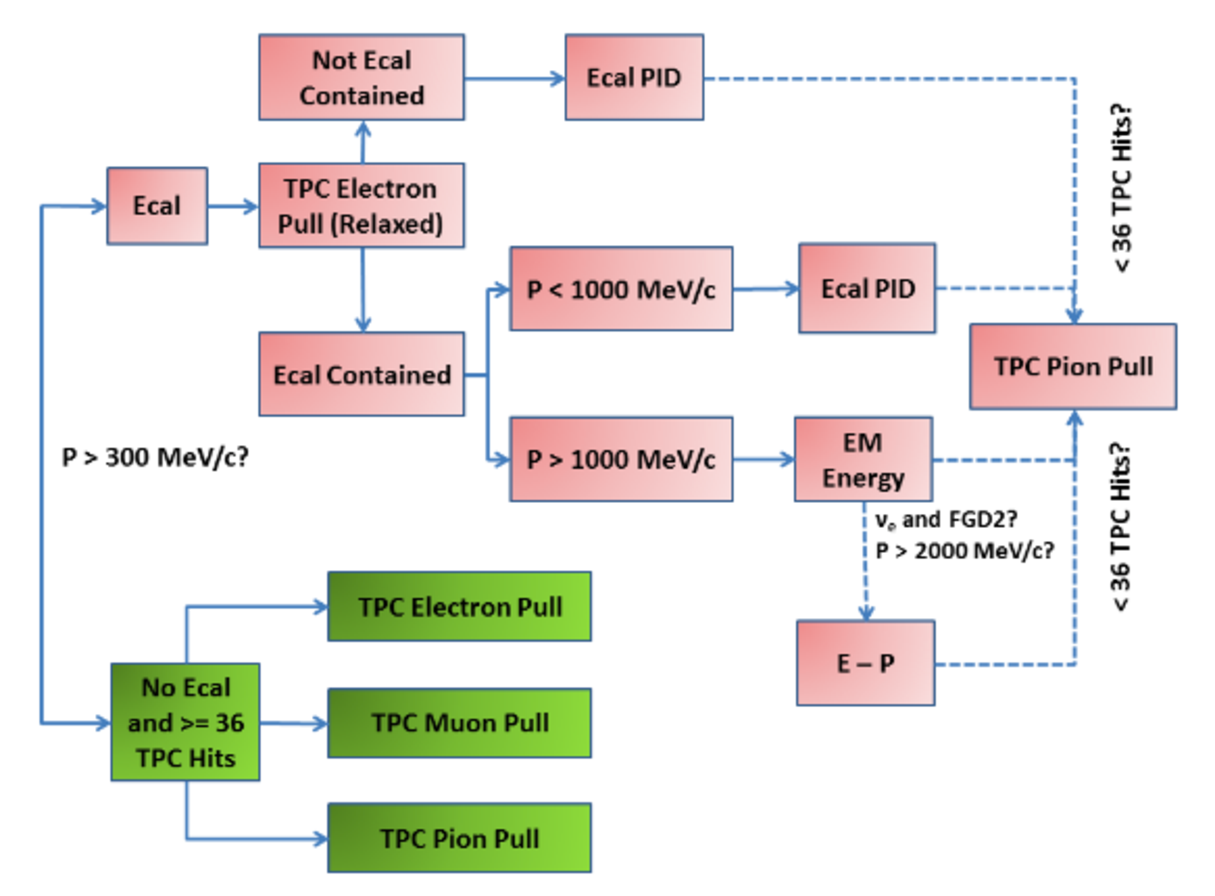
\includegraphics[width=0.8\textwidth]{images/BANFF/NuEPID.pdf} \\
  \caption[The flow chart for the $\nu_e$ PID]{The flow chart for the
    (anti-)\Gls{nue} \Gls{CC} inclusive selections \gls{PID},
    from~\cite{TN282}.}
  \label{fig:NuEPID}
\end{figure}

In Figure~\ref{fig:NuEPID}, one can see that if the track does not
enter the \Gls{ECal} (green boxes), there are three \Gls{TPC}
\Gls{PID} cuts that have been satisfied. They are the following:
\begin{itemize}[noitemsep,topsep=0pt]
\item $-1<\pi_{e, \text{PID}} < 2$,
\item $\pi_{\mu, \text{PID}} \notin \left[-2.5;2.5\right]$
\item and $\pi_{\pi, \text{PID}} \notin \left[-2.5;2.5\right]$.
\end{itemize}

In the case where the track enters the \Gls{ECal}, it must have a
momentum greater than $300$~MeV to be correctly reconstructed in the
\Gls{ECal}. Firstly, the track is required to satisfy a relaxed
\Gls{TPC} \Gls{PID} ($-2<\pi_{e,\text{PID}} < 2.5$). Then,
according to the momentum of the track, the \Gls{ECal} can be used to
provide a \Gls{PID}:
\begin{itemize}[noitemsep,topsep=0pt]
\item The track is tagged as an electron if: (1), the track has a
  momentum greater than $1000$~MeV (2), the \Gls{ECal} reconstructed
  energy is greater than $1100$~MeV and (3), the shower is fully
  contained in the \Gls{ECal}.
\item In the case where one of the conditions above is not satisfied,
  the \Gls{PID} quantity \Gls{MIPEM}\footnote{The \Gls{MIPEM} quantity
    is an \Gls{ECal} reconstructed variable related to the topology of
    the particle. It is the discriminator of a boosted decision tree
    on the \Gls{ECal} object variables. This tree was trained electron
    and muon particle guns, and therefore aims at differentiating
    \Gls{MIP}-like object and \Gls{EM} showers.} has to be greater
  than 0.
\end{itemize}

Another special case is when the track was selected in the
\Gls{FGD}2. In that case, it was noted that there are still many muons
after the selection, therefore another cut was made using a combined
variable of \Gls{TPC} and \Gls{ECal} which is defined as $E-p$. This
variable has to be greater than $-2000$~MeV for the event to pass the
selection.

\subsubsection{Second \Gls{TPC} \Gls{PID}}
\label{subsubsec:secondtpcpid}
If the track is from \Gls{FGD}1 and propagates until the \Gls{TPC}3,
then another \Gls{PID} is realised with it:
\begin{itemize}[noitemsep,topsep=0pt]
\item in the case of electron neutrino selection, the requirement is
  $-2.5<\pi_{e, \text{PID}} < 2.5$;
\item in the case of electron anti-neutrino selection, the requirement
  is $-3<\pi_{e, \text{PID}} < 3$, but is only applied in the region
  where the proton $dE/dx$ overlaps (positron momentum between $600$
  and $1650$~MeV).
\end{itemize}

\subsubsection{Proton \Gls{PID}}
In the case of electron anti-neutrino selection, there is still a
large contamination of protons for track of momentum greater than
$600$~MeV.  Another hybrid \Gls{TPC}~/~\Gls{ECal} variable is
therefore constructed ($E/p$), and the following requirements are
made:
\begin{itemize}[noitemsep,topsep=0pt]
\item if $p<1650$~MeV, $E/p > 0.65$,
\item if $p>1650$~MeV, $E/p > 0.15$,
\end{itemize}
Then, another \Gls{ECal} \Gls{PID} cut is made on the quantity
\Gls{EMHIP}\footnote{Similar to \Gls{MIPEM}, this variable is the
  discriminator variable of a boosted decision the tree on the
  \Gls{ECal} object variable. This tree was trained on a proton and
  electrons particle guns and therefore aims at differentiating
  hadronic-like object and \Gls{EM} showers.}. This variable has to be
negative.

\subsubsection{\Gls{TPC} veto}
This cut is the same as the one described in
Section~\ref{subsec:muonneutrinoselection}, except the difference
in distance is $100$~mm rather than $150$~mm.

\subsubsection{Photon veto}
One of the problem with these samples is the presence of a large
photon background in the first bins of the electron (or positron)
momentum, this background has very similar characteristics to the one
observed in Chapter~\ref{chap:select}. This is the reason why a
constraint from the photon sample was introduced to reduce the
uncertainty on these backgrounds.

If there is a second track of opposite charge, with a number of
\Gls{TPC} nodes greater than $18$, and a \Gls{PID} satisfying:
$-3<\pi_{e, \text{PID}} < 3$, and if the system's invariant mass
(Equation~(\ref{eq:invariantmass})) is smaller than $100$~MeV, and
starts at a distance smaller than $100$~mm, the event is rejected.

\subsubsection{\Gls{PD}, \Gls{P0DECal} and \Gls{FGD}1 veto}
If there is any upstream activity in the \Gls{PD} or \Gls{P0DECal},
the event is rejected. If the event was in \Gls{FGD}2, any activity in
the \Gls{FGD}1 results in the vetoing of the event.

\subsubsection{\Gls{ECal} veto}
The \Gls{ECal} veto aims at rejecting the \Gls{OOFV} events. However,
it is applied differently from the one described in
Section~\ref{subsec:singlephotonselection}, due to the complexity of
the \Gls{ECal} \Gls{PID} as described before. In this case, only
upstream events are vetoed, and the selected event is rejected if an
object starts at a distance greater than $100$~mm in the upstream
direction.

\subsubsection{FGD2 shower}
\label{subsubsec:fgd2shower}
This cut is only applied to electron anti-neutrino selection which
have tracks of momentum greater than $600$~MeV. Positrons coming from
\Gls{FGD}1 can shower in the \Gls{FGD}2, and produce several tracks in
the \Gls{TPC}3.

Note that this cut is realised since there is still a large proton
contamination in this sample. Firstly, the track is required to go the
\Gls{FGD}2, then, the number of matched tracks from
\Gls{FGD}1-\Gls{TPC}2 has to be greater than \Gls{FGD}2-\Gls{TPC}3
matched tracks.

The criteria on the number of \Gls{FGD}2-\Gls{TPC}3 tracks are applied
and the event is rejected if:
\begin{itemize}[noitemsep,topsep=0pt]
\item There are two or less \Gls{FGD}2-\Gls{TPC}3 tracks in the proton
  momentum region ($600 < p < 1650$), or one or less
  \Gls{FGD}2-\Gls{TPC}3 tracks in high energy region ($p > 1650$~MeV),
  as the high energy tail is less contaminated with the proton
  background.
\item Only applied to tracks where the second \Gls{TPC} \Gls{PID} has
  not been applied: in the proton momentum region ($600 < p < 1650$),
  if there is at least one secondary \Gls{FGD}1-\Gls{TPC}2 track and
  there are three or less \Gls{FGD}2-\Gls{TPC}3 tracks. This cut is
  applied to reduce reconstruction effects (such as the
  \Gls{FGD}-\Gls{TPC} matching failures) and deals with secondary
  tracks showering in \Gls{FGD}2.
\end{itemize}

\section{Systematic uncertainties}
\label{subsec:systematicsbanff}
In this analysis, the errors are the parameters of interest, however
this is a Bayesian analysis, therefore they have some prefit values
and errors, which enclose the ``best guesses'' for these values. Each
of them is detailed here, starting with the flux, then the cross
section and finally the detector systematic uncertainties.

\subsection{Flux error}
\label{subsec:fluxsyst}
The description of this systematic error can be found in
Section~\ref{sec:fluxsyst}.

\subsection{Cross section error}
\label{subsec:xsecsystccqe}
The cross section systematic errors evaluations are relying on the use
of external data sets. In this section, only the parameters related to
the \Gls{CCQE}-like events that have not already been used in
Section~\ref{sec:xsecsyst}\footnote{Two marginal differences ought to
  be noted, the parameter controlling the $\Delta$ resonance mass is
  not used here, since it is more related to the ``hadronic side'' or
  the interaction and the pion momentum distributions; and the
  \Gls{NC} \Gls{COH} uncertainty is $30\%$ (the \Gls{CC} is still
  $100\%$).} are described.


\subsubsection{Long range correlations}
\label{subsubsec:lrc}
The long range correlations refer to the one of the corrections listed
in Section~\ref{subsec:ccqe}, their effects is on the $Q^2$ quantity:
at low $Q^2$ the cross section is expected to be reduced; whereas it
is enhanced at intermediate $Q^2$ and goes back to unity for
$Q^2\rightarrow \infty $. This can be seen in Figure~\ref{fig:BeRPA},
which shows the central value and error envelope
from~\cite{NievesCCinc}.

\begin{figure}[ht]
  \center
  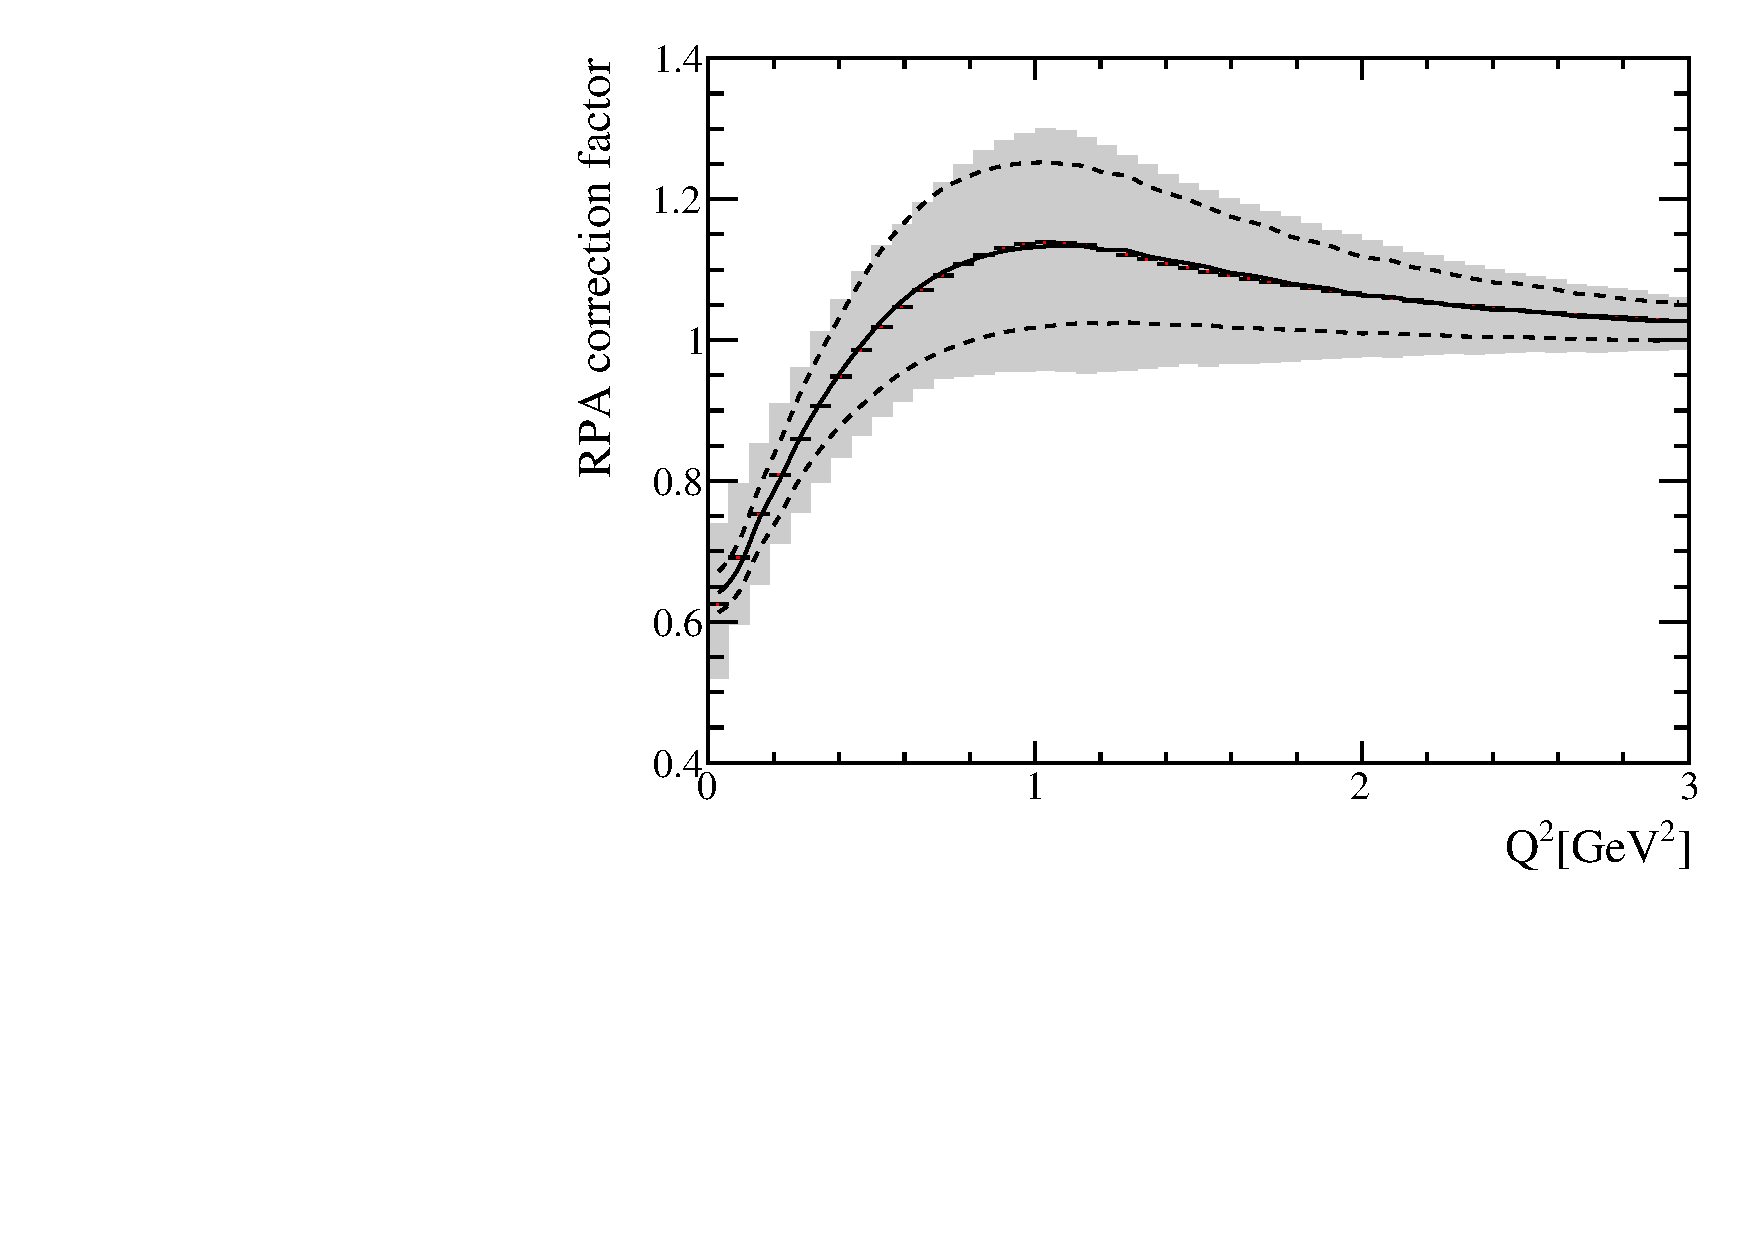
\includegraphics[width=0.6\textwidth]{images/BANFF/erpa_20percent_combined_throws}
  \caption[BeRPA corrections and errors]{The \Gls{BeRPA}
    corrections and errors, from Nieves et al.~\cite{NievesCCinc}
    (black solid line for the central value and dotted line for the
    error) and the ones used in \Gls{TK} (black data points for the
    central value and grey band for the error, as shown in
    Table~\ref{tab:BeRPA}); from~\cite{TN315}.}
  \label{fig:BeRPA}
\end{figure}

For \Gls{TK} analysis, the effects are parametrised through a weight
which takes $Q^2$ as a parameter and is called the e\Gls{RPA} (for
effective Random Phase Approximation). Since a simple parametrisation
via polynomials led to complex correlations between its parameters,
the formalism was developed in a Bernstein polynomial basis (and the
correction is therefore referred as \Gls{BeRPA} within \Gls{TK}). The
weighting function is defined as:

\begin{equation*}
  \label{eq:BeRPA}
  f(Q^2) = 
  \begin{cases}
    A(1-\frac{Q^2}{U})^{3} + 3B(1-\frac{Q^2}{U})^{2}\left(\frac{Q^2}{U}\right) + 3p_{1}(1-\frac{Q^2}{U})\left(\frac{Q^2}{U}\right)^{2} + C\left(\frac{Q^2}{U}\right)^{3}, & Q^2 < U \\
    1 + p_{2}\exp(Q^2p(-D(Q^2-U)), & Q^2 > U,
  \end{cases}
\end{equation*}
where $A$, $B$, $C$ and $p_1$ are the normalisation parameters of each
Bernstein polynomial. $U$ is the value for which the parametrisation
becomes exponential for which $D$ is the damping parameter.  Note that
continuity between the two parts of this equation leads to a non
trivial relation between the parameters:

\begin{align*}
  \label{eq:BeRPAcont}
  p_{1} &= C + \frac{UD(C-1)}{3}\\
  p_{2} &= C - 1
\end{align*}

The fit to the \Gls{RPA} corrections from~\cite{NievesCCinc} and an
{\it ad hoc} choice of errors are listed in Table~\ref{tab:BeRPA}.

\begin{table}[h!]
  \center
  \begin{tabular}{ccc}
    \toprule
    Parameter & Nominal value & Uncertainty \\ 
    \midrule
    $A$ &  $0.59$ & $20\%$ \\
    $B$ &  $1.05$ & $20\%$ \\
    $C$ &  $1.13$ & $15\%$ \\
    $D$ &  $0.88\text{~GeV}^2$ & $40\%$ \\
    $U$ &  $1.20\text{~GeV}^2$ & fixed \\
    \bottomrule
  \end{tabular}
  \caption[Nominal values and uncertainties for the five BeRPA
  parameters]{Nominal values and uncertainties for the five
    \Gls{BeRPA} parameters. Note that $U$ should not be varied and no
    uncertainty is provided. All the parameters must be positive and
    are uncorrelated between them. Reproduced from~\cite{TN315}.}
  \label{tab:BeRPA}
\end{table}


\subsubsection{Multi nucleons error parametrisation}
As can be seen in Figure~\ref{fig:xsecs_plot} (which shows integrated
neutrino cross section on carbon as function of energy), multi nucleon
processes are expected to have a major impact on oscillation analyses
at \Gls{TK}~\cite{MartiniERec}. The normalisation and shape of the
cross section can be changed within the \Gls{BANFF}. The
normalisations are changed based on the (anti-) neutrino type
(\gls{numu}, \gls{anumu}, \gls{nue} and \gls{anue}) and target (carbon
or oxygen).

Since the multi nucleon cross section can be separated into two
components, the Delta resonance and the \gls{2p2h} contributions, the
shape uncertainty is determined by running the code from Nieves et
al.~\cite{NievesCCinc} with the contributions seperately and adopting
a reweighting scheme that takes care of the interferences between them
(note that the total cross section is maintained constant to avoid
interfering with the other normalisation parameters). The illustration
of the shape change is shown in Figure~\ref{fig:2p2herror}. The
reweighting scheme is done in three dimensions: neutrino energy,
momentum and energy transfer ($E_\nu$, $q_3$ and $q_0$, respectively).

\subsubsection{CCQE and multi nucleon errors}
The \Gls{CCQE} form factor extracted from bubble chamber
data\cite{ANLCCQE,BNLCCQE,CERNCCQE} does not reproduce \Gls{TK}
data. Similarly this applies to the Fermi momentum in the nucleus and
the multi-nucleon errors derived from
\Gls{MiniBooNE}~\cite{MiniBooNENuCCQE} and
\Gls{MINERVA}~\cite{MinervaNuCCQE}, experiments. Therefore, there is
no prior for these quantities.

\begin{figure}[ht]
  \begin{adjustbox}{center}
    \begin{tabular}{cc}
      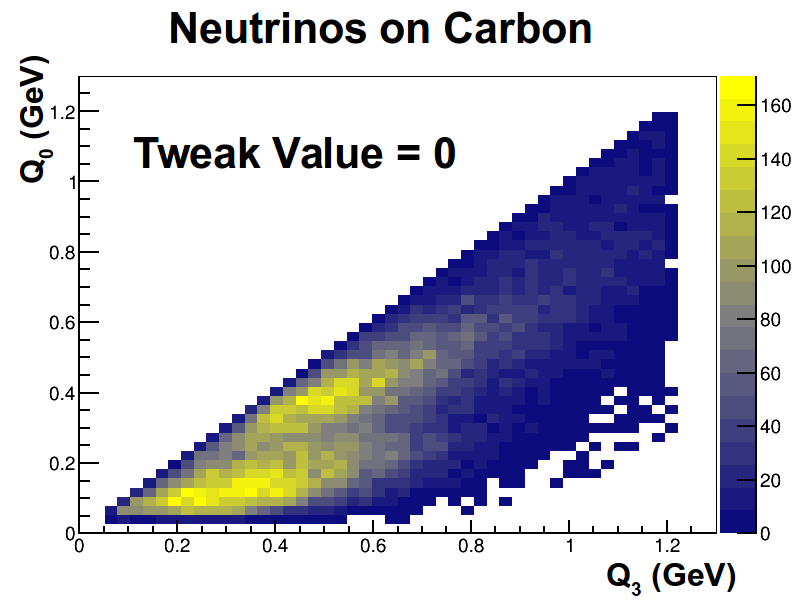
\includegraphics[width=0.48\textwidth]{images/BANFF/neutrino_carbon_0.png} &\\
      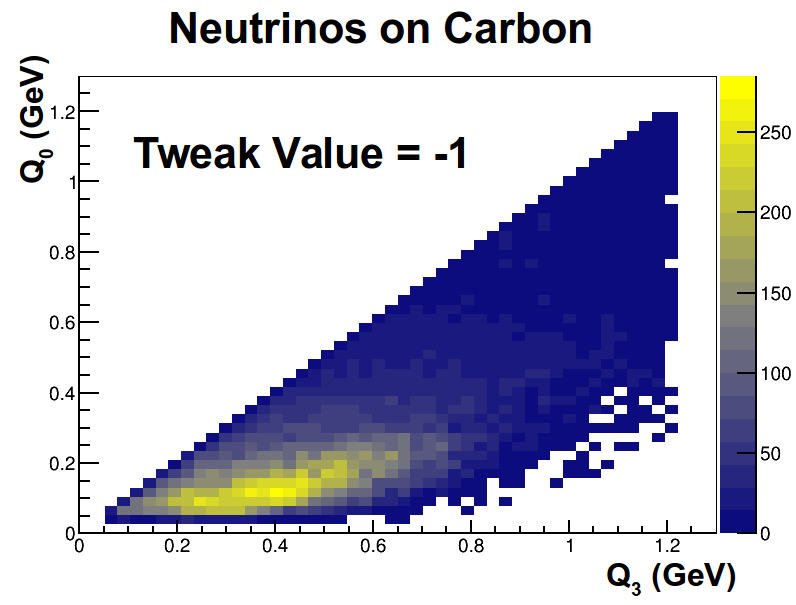
\includegraphics[width=0.48\textwidth]{images/BANFF/neutrino_carbon_m3.png}&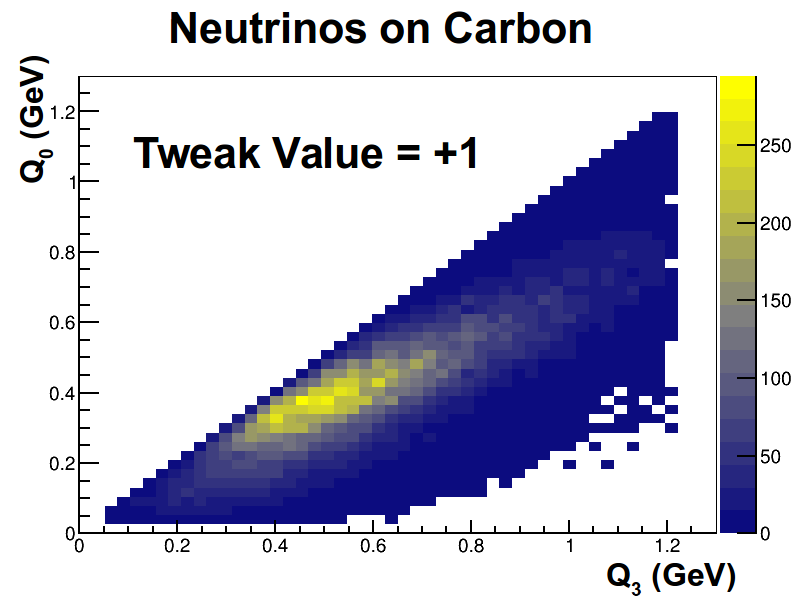
\includegraphics[width=0.48\textwidth]{images/BANFF/neutrino_carbon_p3.png}
    \end{tabular}
  \end{adjustbox}
  \begin{center}
    \caption[Effect of change in the multi nucleon parameters]{Effect
      of change in the multi nucleon parameters for $q_3$, $q_0$, for
      all the \Gls{ND}. \textbf{\textit{Top:}}
      Nominal. \textbf{\textit{Bottom left:}} $-1\sigma$ variation.
      \textbf{\textit{Bottom right:}} $+1\sigma$ variation.
      From~\cite{TN315}.}
    \label{fig:2p2herror}
  \end{center}
\end{figure}

\subsubsection{Final state interaction error}
Unlike what is described in Section~\ref{subsec:fsiuncertainty}, the
\Gls{FSI} uncertainty is parametrised as continuous parameters, which
allows to simply fit them. Note that the \Gls{FSI} parameters are not
propagated to \Gls{SK} and therefore are purely nuisance
parameters. The systematic error are the same as what was described in
Section~\ref{subsec:fsiuncertainty}.

\subsubsection{Electron neutrino error}
The error described in Section~\ref{subsec:electnuerror} is smaller
than the errors that are found when measuring the electron neutrino
cross sections (let alone the electron anti-neutrinos!). It seems that
this theory-driven approach is a fairly dangerous way of estimating
the error on the \Gls{CP} violation signal. For this analysis, the
errors are inflated to the somewhat arbitrary 140\% (and no
correlation) which is well beyond the expected sensitivity of the
electron neutrino samples. For example, the fact that the electron
neutrino has a smaller mass opens different areas of the parameter
space in very low $Q^2$ regions, for example.

\subsubsection{Prefit correlation matrix}
Finally, the prefit correlations are shown in
Figure~\ref{fig:asimovprefitxsec}. This correlation matrix is created
``by hand,'' using {\it ad hoc} correlations. For example, in the case
of \Gls{2p2h}-shape on carbon and oxygen, the correlation is $50\%$
based on discussions with theorists~\cite{NievesCorrelations}. Some of
the other correlations come from data, namely the resonant parameters
correlations come from bubble chamber data analysis, and the \Gls{FSI}
parameters ones come from pion scattering data analysis. For the rest
of the \Gls{CCQE} parameters, no correlations are assumed, this is
because \Gls{TK} is very sensitive to the these processes and usually
produces a bad fit if correlations are included in the prefit
matrix. This means that the \Gls{TK} data is not compatible with the
\Gls{MiniBooNE} and \Gls{MINERVA} data within our models.

Note that, as mentioned in the previous section and visible in the
Figure~\ref{fig:asimovprefitxsec}, the correlation between the
$\nu_{e}/\nu_{\mu}$ and its equivalent in for anti-neutrino has been
set to zero.

\begin{figure}[ht]
  \center
  \includegraphics[width=0.9\textwidth,page=3]{images/BANFF/OutputAsimov_matrices.pdf}\\
  \begin{center}
    \caption[The prefit error correlations for the cross section
    uncertainties]{The prefit error correlations for the cross section
      uncertainties.}
    \label{fig:asimovprefitxsec}
  \end{center}
\end{figure}

\subsection{Detector, Monte Carlo statistics and 1p1h error}
As for the \Gls{FSI}, the detector errors are ``nuisance'' parameters
and are not propagated to \Gls{SK}. The error is parametrised using a
covariance matrix. This covariance matrix is built by throwing ``toy
experiments'' according to a binning similar to the one used for the
fit (which is detailed in Appendix~\ref{app:binning}), but coarser
(note that there are $1438$ bins in the fit, and if one used of the
full matrix, the fit would become unacceptably long, the reduced
binning brings the number of bins to $542$). The fit is then allowed
to change the overall normalisation of a bin in a coherent way
according to the detector errors. Most of the systematic uncertainties
that are relevant are the same as the one listed in
Section~\ref{sec:detsyst}, note that the \Gls{OOFV} normalisation that
was described in that section was not applied during the construction
of the covariance matrix. Rather, a symmetric, Gaussian uncertainty of
$30\%$ was used. In this case, the photon sample acts as a control
sample for the \gls{nue} samples and the \Gls{OOFV} error is
correlated between the electron samples. The correlations and diagonal
errors are shown in Figure~\ref{fig:ndcov}.

Note that all the figures in this section are organised with the order
for the samples in Table~\ref{tab:samples}, (left to right and down to
up in the matrix, with the detector binning from
Appendix~\ref{app:binning}, with each momentum bin being inside a
cosine bin).

\begin{table}
  \begin{adjustbox}{center}
    \begin{tabular}{cccccc}
      \toprule
      \multirow{3}{*}{Horn current} & \multirow{3}{*}{\Gls{FGD}} & \multirow{3}{*}{Topology}     & \multicolumn{3}{c}{Number of bins}           \\
                                    &                            &                               & \multicolumn{3}{c}{in the fit (covariance)}  \\
                                    &                            &                               & Momentum & $\cos(\theta)$ & Total            \\
      \midrule
      \Gls{FHC}                     & 1                          & \Gls{numu} \Gls{CC} 0 pion    & 14 (6)    & 11  (7)       & 154 (42)         \\ 
      \Gls{FHC}                     & 1                          & \Gls{numu} \Gls{CC} 1 pion    & 13 (5)    & 11  (8)       & 143 (40)         \\ 
      \Gls{FHC}                     & 1                          & \Gls{numu} \Gls{CC} other     & 14 (5)    & 11  (8)       & 154 (40)         \\ 
      \Gls{FHC}                     & 2                          & \Gls{numu} \Gls{CC} 0 pion    & 14 (6)    & 11  (7)       & 154 (42)         \\ 
      \Gls{FHC}                     & 2                          & \Gls{numu} \Gls{CC} 1 pion    & 13 (5)    & 11  (8)       & 143 (40)         \\ 
      \Gls{FHC}                     & 2                          & \Gls{numu} \Gls{CC} other     & 14 (5)    & 11  (8)       & 154 (40)         \\ 
      \Gls{FHC}                     & 1                          & \Gls{nue} \Gls{CC} inclusive  &  6 (6)    &  3  (1)       &  18  (6)         \\ 
      \Gls{FHC}                     & 2                          & \Gls{nue} \Gls{CC} inclusive  &  6 (6)    &  3  (1)       &  18  (6)         \\ 
      \Gls{RHC}                     & 1                          & \Gls{numu} \Gls{CC} 0 pion    &  6 (4)    &  7  (7)       &  42 (28)         \\ 
      \Gls{RHC}                     & 1                          & \Gls{numu} \Gls{CC} 1 pion    &  8 (4)    &  4  (4)       &  32 (16)         \\ 
      \Gls{RHC}                     & 1                          & \Gls{numu} \Gls{CC} other     &  6 (4)    &  3  (3)       &  18 (12)         \\ 
      \Gls{RHC}                     & 2                          & \Gls{numu} \Gls{CC} 0 pion    &  6 (4)    &  7  (7)       &  42 (28)         \\ 
      \Gls{RHC}                     & 2                          & \Gls{numu} \Gls{CC} 1 pion    &  8 (8)    &  4  (4)       &  32 (32)         \\ 
      \Gls{RHC}                     & 2                          & \Gls{numu} \Gls{CC} other     &  6 (4)    &  3  (3)       &  18 (12)         \\ 
      \Gls{RHC}                     & 1                          & \Gls{anumu} \Gls{CC} 0 pion   &  8 (4)    & 10 (10)       &  80 (40)         \\ 
      \Gls{RHC}                     & 1                          & \Gls{anumu} \Gls{CC} 1 pion   &  6 (4)    &  3  (3)       &  18 (12)         \\ 
      \Gls{RHC}                     & 1                          & \Gls{anumu} \Gls{CC} other    &  8 (4)    &  4  (4)       &  32 (16)         \\ 
      \Gls{RHC}                     & 2                          & \Gls{anumu} \Gls{CC} 0 pion   &  8 (4)    & 10 (10)       &  80 (40)         \\ 
      \Gls{RHC}                     & 2                          & \Gls{anumu} \Gls{CC} 1 pion   &  6 (6)    &  3  (3)       &  18 (18)         \\ 
      \Gls{RHC}                     & 2                          & \Gls{anumu} \Gls{CC} other    &  8 (4)    &  4  (4)       &  32 (16)         \\ 
      \Gls{RHC}                     & 1                          & \Gls{nue}  \Gls{CC} inclusive &  6 (6)    &  2  (1)       &  12  (6)         \\ 
      \Gls{RHC}                     & 2                          & \Gls{nue}  \Gls{CC} inclusive &  6 (6)    &  2  (1)       &  12  (6)         \\ 
      \Gls{RHC}                     & 1                          & \Gls{anue} \Gls{CC} inclusive &  3 (3)    &  2  (1)       &   6  (3)         \\ 
      \Gls{RHC}                     & 2                          & \Gls{anue} \Gls{CC} inclusive &  3 (3)    &  2  (1)       &   6  (3)         \\ 
      \Gls{FHC}                     & 1                          & photon background             &  5 (5)    &  1  (1)       &   5  (5)         \\ 
      \Gls{FHC}                     & 2                          & photon background             &  5 (5)    &  1  (1)       &   5  (5)         \\ 
      \Gls{RHC}                     & 1                          & photon background             &  5 (5)    &  1  (1)       &   5  (5)         \\ 
      \Gls{RHC}                     & 2                          & photon background             &  5 (5)    &  1  (1)       &   5  (5)         \\
      \bottomrule
    \end{tabular}
  \end{adjustbox}
  \caption[Number of bins and ordering in the covariance
  matrices]{Sample-wise number of bins and ordering in the covariance
    matrices.}
  \label{tab:samples}
\end{table}    

\begin{figure}[ht]
  \begin{center}
    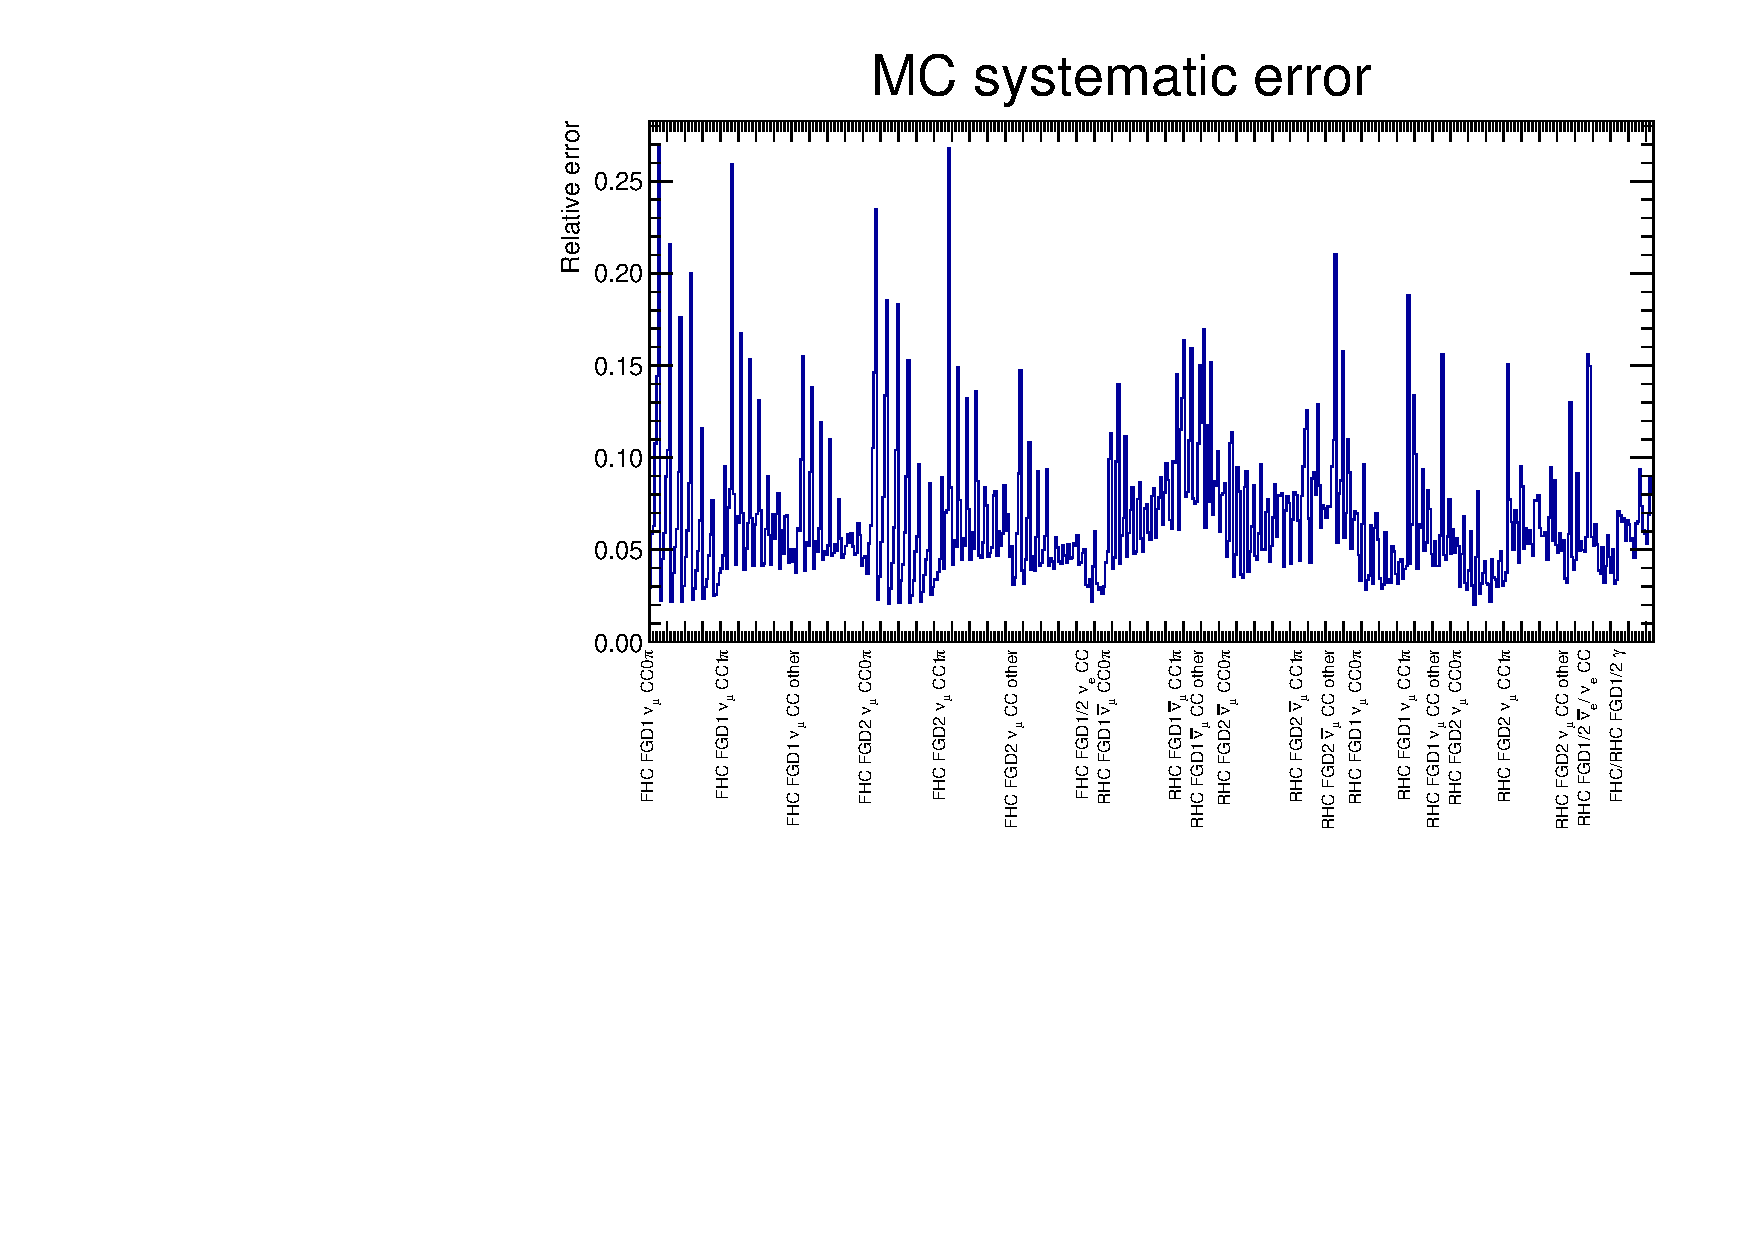
\includegraphics[width=0.78\textwidth]{images/BANFF/mc_sys_error_redu.pdf} \\
    \includegraphics[width=0.78\textwidth]{images/BANFF/CorrDetectorOnly.\extensionimage}
    \caption[Relative detector uncertainties and correlations for the
    lepton reconstructed bins]{\textbf{\textit{Top:}} Relative
      detector uncertainties for each lepton reconstructed bin (square
      root of the diagonal of the covariance matrix).
      \textbf{\textit{Bottom:}} Correlations between the bins. The
      samples are organised as mentioned in Table~\ref{tab:samples}.}
    \label{fig:ndcov}
  \end{center}
\end{figure}

The \Gls{MC} statistical errors should not be propagated to \Gls{SK},
therefore the inverse of square root of the number of entries of the
Monte Carlo histograms is added in quadrature to the diagonal of the
covariance matrix to take it into account. The \Gls{MC} statistical
relative errors are shown in Figure~\ref{fig:mcstaterror}.

\begin{figure}[ht]
  \begin{center}
    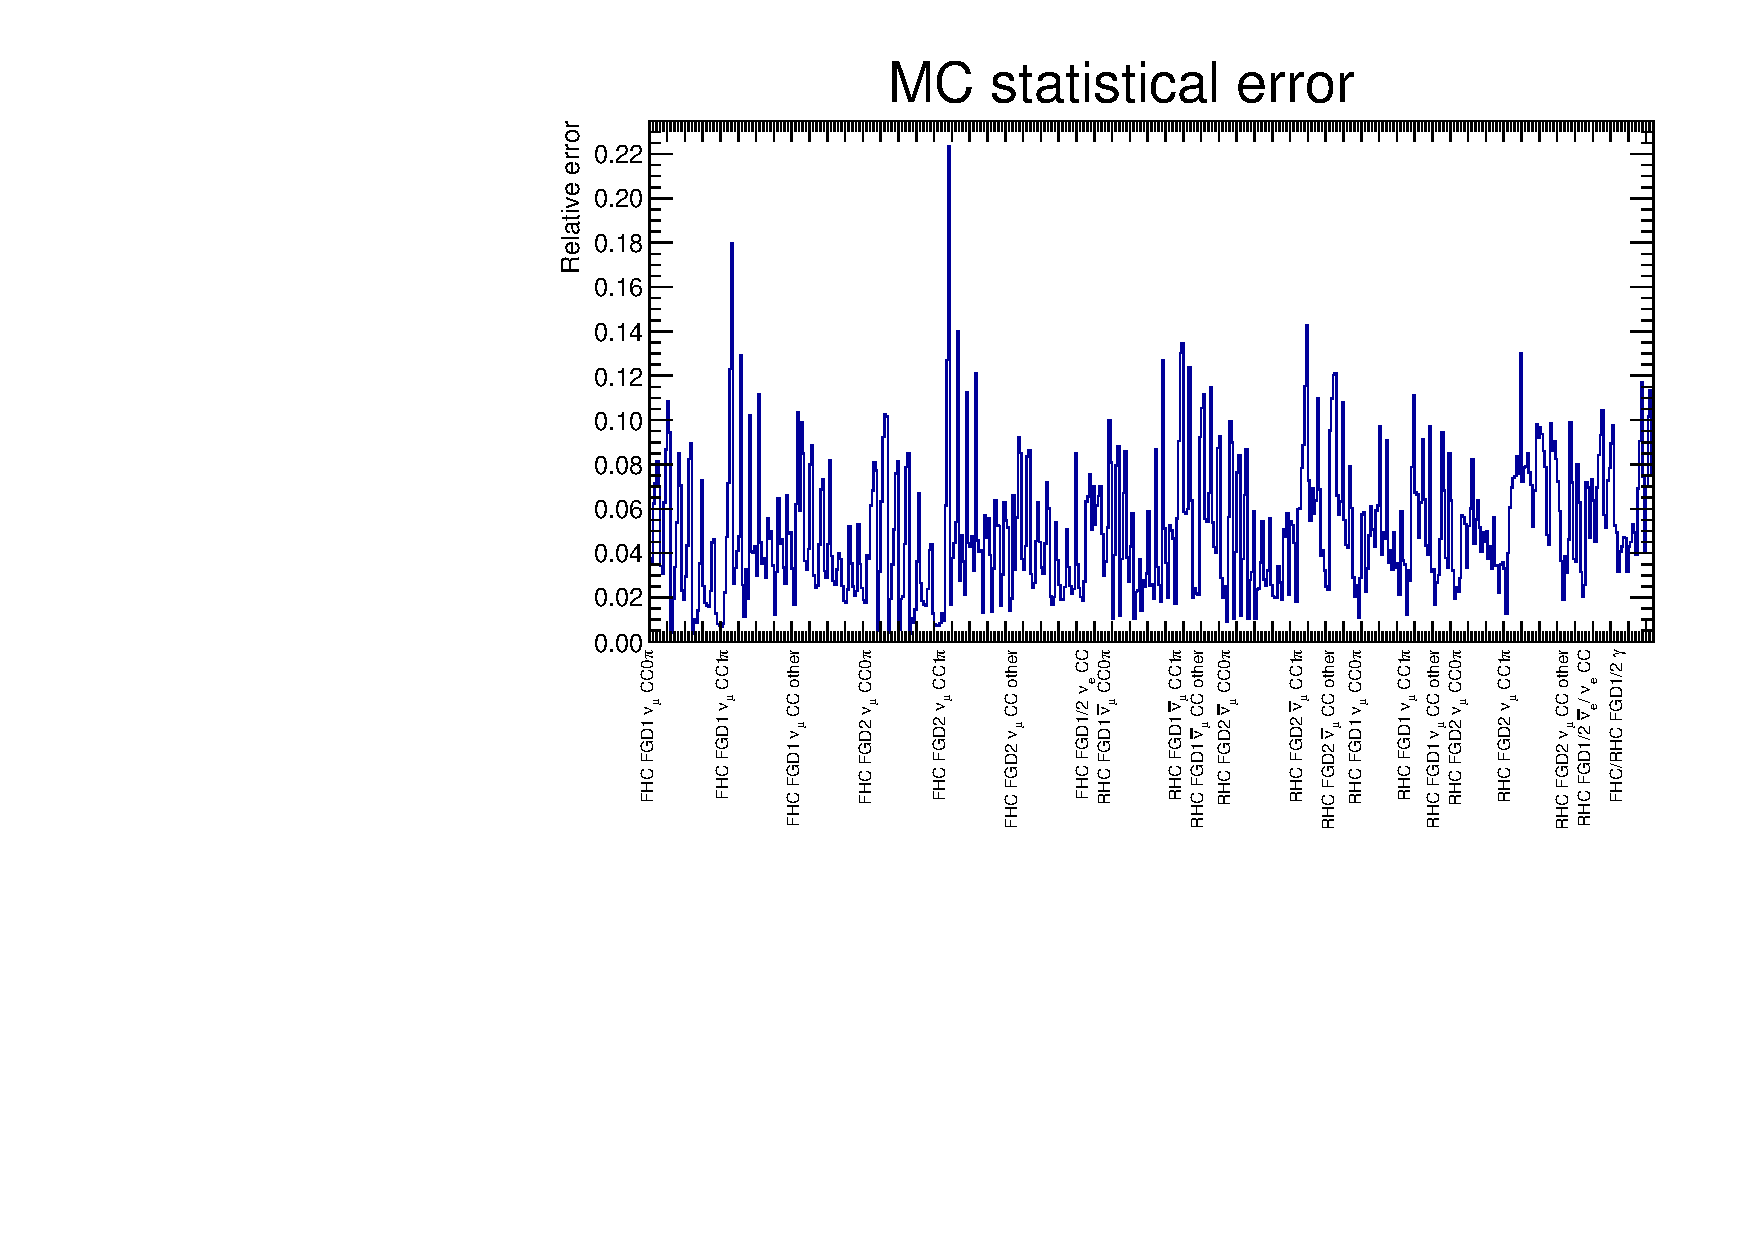
\includegraphics[width=0.78\textwidth]{images/BANFF/mc_stat_error_redu.pdf}
    \caption[Monte Carlo statistical uncertainty for the lepton
    reconstructed bins]{Monte Carlo statistical uncertainty for the
      lepton reconstructed bins. The samples are organised as mentioned
      in Table~\ref{tab:samples}.}
    \label{fig:mcstaterror}
  \end{center}
\end{figure}

Finally, some cross section errors have not been fully implemented
yet, and the \Gls{TK} collaboration only has access to differences
between the \Gls{NEUT} and the Nieves et al. model~\cite{NievesCCinc}
for the propagation of the 1p1h error. In this case, since one cannot
parametrise properly the difference between the two models, a ``fake
data'' is created and the difference between the two models is added
to the covariance matrix, assuming full correlations for the
differences of models. This allows to have a smooth transition between
the \Gls{NEUT} and Nieves models via the covariance matrix. The fake
data relative errors are shown in Figure~\ref{fig:fakedataerror}.

\begin{figure}[ht]
  \center
  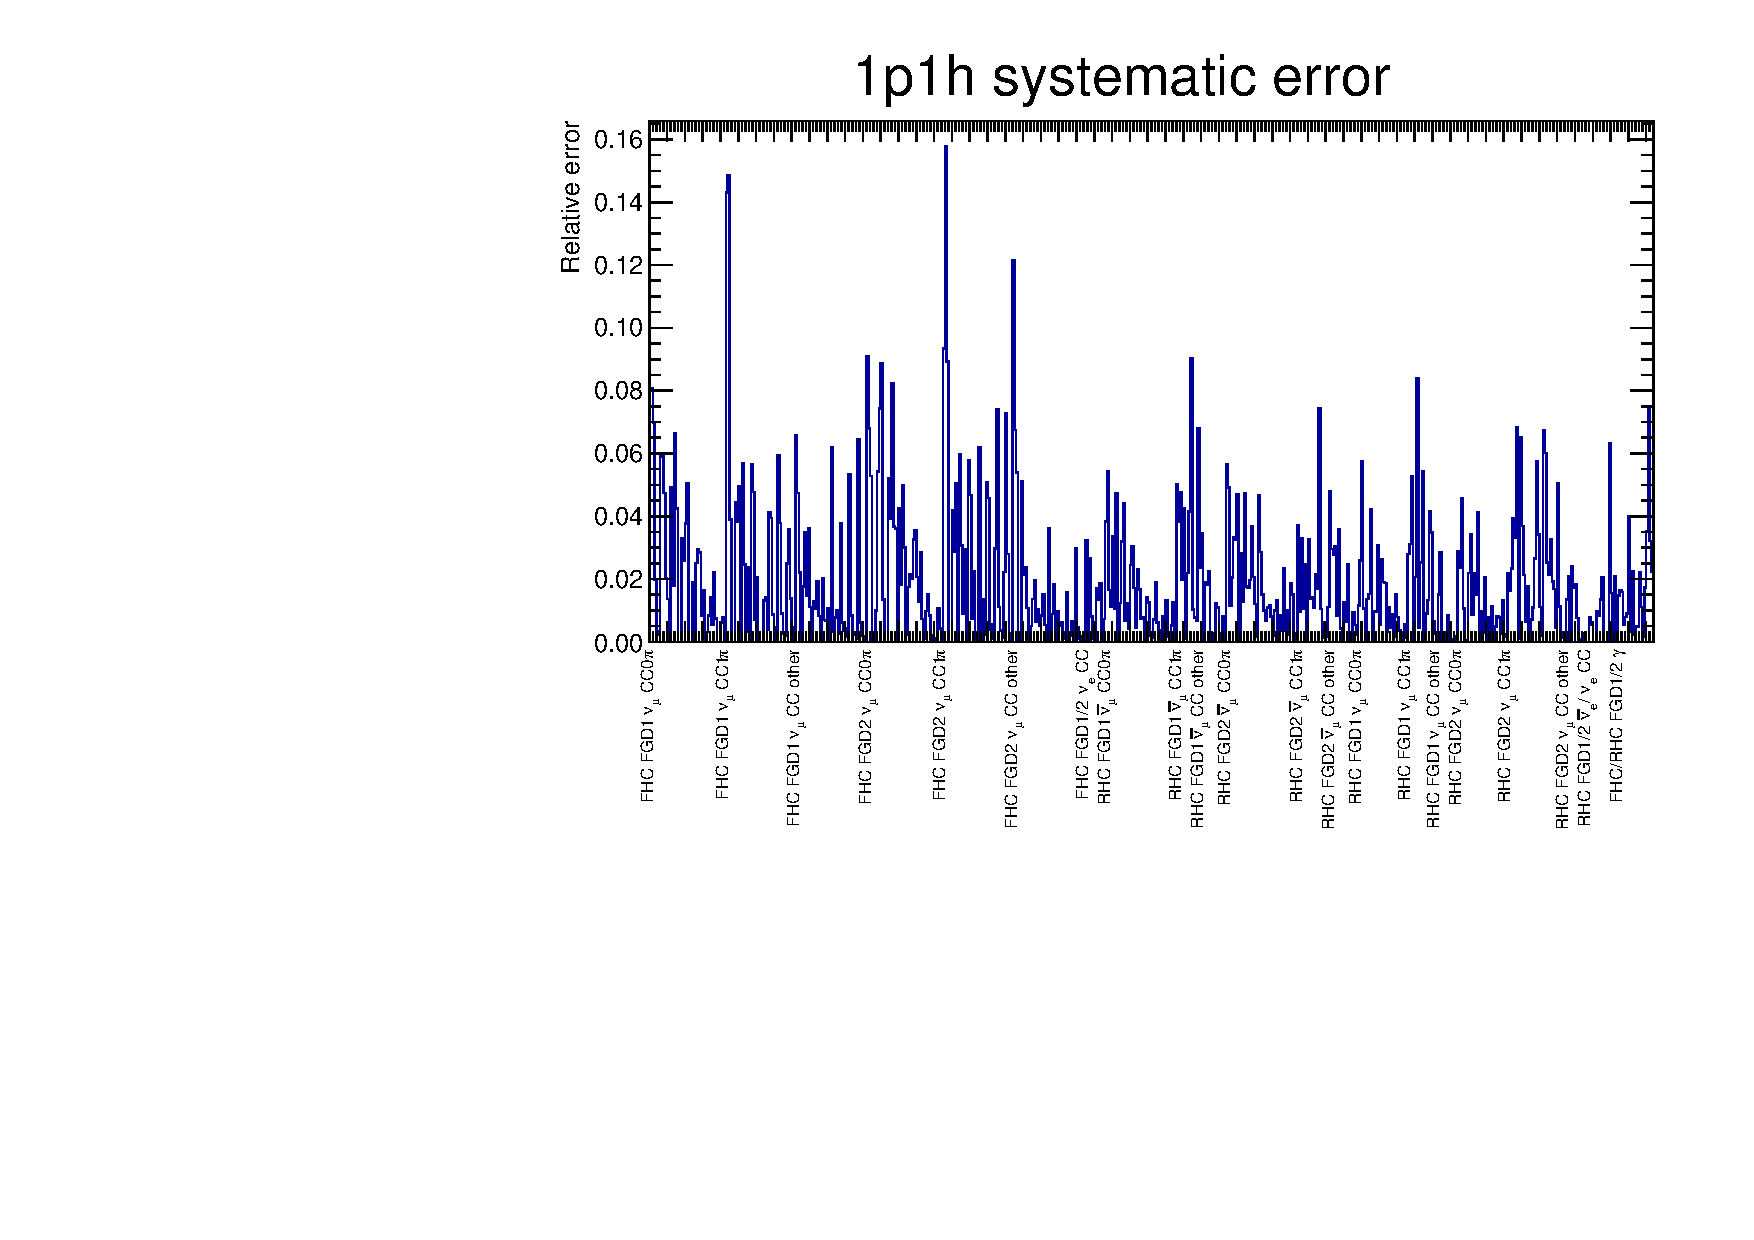
\includegraphics[width=0.78\textwidth]{images/BANFF/1p1h_fake_Error_redu.pdf} \\
  \includegraphics[width=0.78\textwidth]{images/BANFF/CorrFakeOnly.\extensionimage}
  \caption[1p1h fake data error and correlations for the lepton
  reconstructed bins]{\textbf{\textit{Top:}} 1p1h fake data error for
    the lepton reconstructed bins. \textbf{\textit{Bottom:}}
    Correlations between the bins ($100\%$, $-100\%$ or $0\%$). The
    samples are organised as mentioned in Table~\ref{tab:samples}.}
  \label{fig:fakedataerror}
\end{figure}

The addition of the detector, \Gls{MC} statistical and 1p1h fake data
errors are shown in Figure~\ref{fig:totndcov}. Note that when the
covariance is constructed, the detector systematic uncertainties
produce shifts due to their non gaussianity. To take this into
account, the normalisation of each bin is shifted according to the
mean value of the toys observed in each bin. These ``bin shifts'' can
be found in Figure~\ref{fig:totndcovshift}.

\begin{figure}[ht]
  \center
  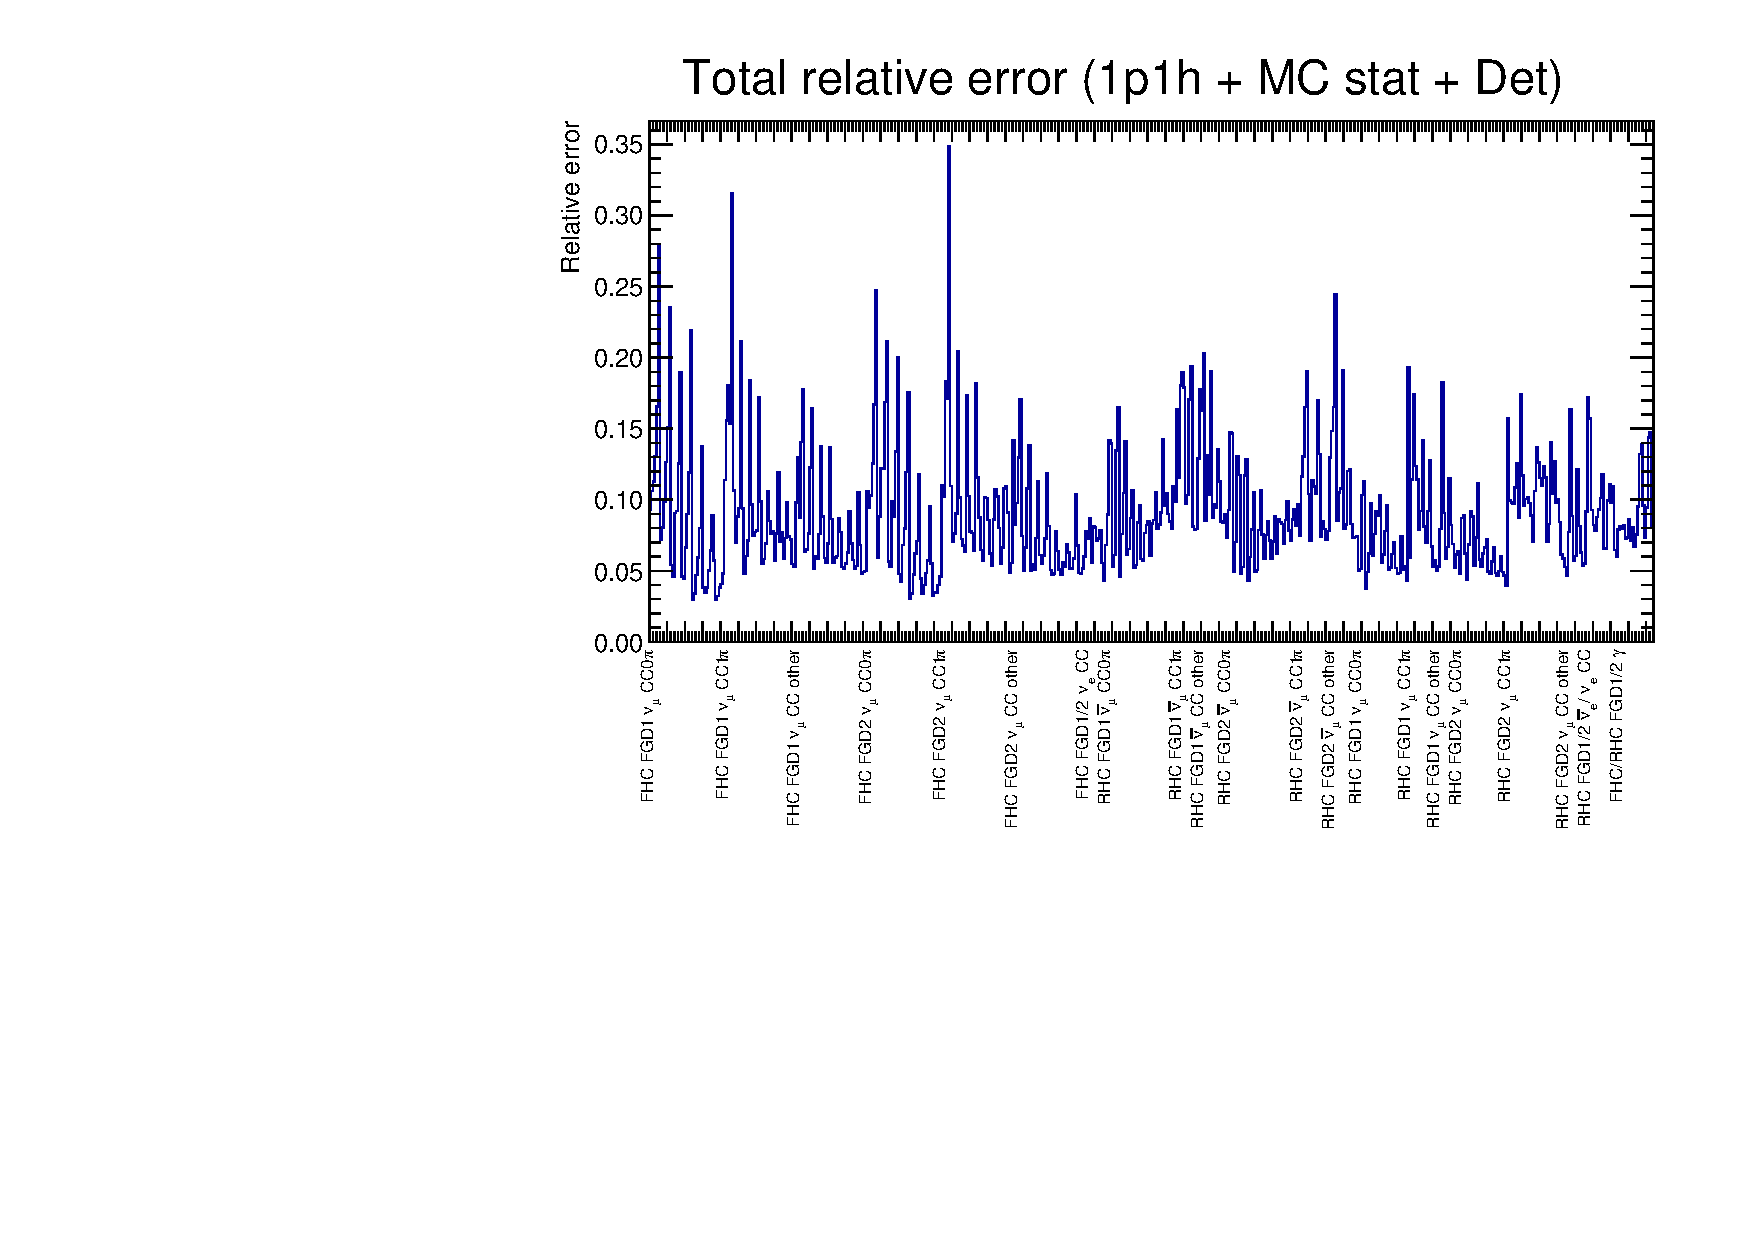
\includegraphics[width=0.78\textwidth]{images/BANFF/totalerr.pdf} \\
  \includegraphics[width=0.78\textwidth]{images/BANFF/CorrTotal.\extensionimage}
  \caption[Total error and correlations for the lepton reconstructed
  bins]{\textbf{\textit{Top:}} Total error for the lepton
    reconstructed bins. \textbf{\textit{Bottom:}} Correlations between
    bins. The samples are organised as mentioned in
    Table~\ref{tab:samples}.}
  \label{fig:totndcov}
\end{figure}

\begin{figure}[ht]
  \center
  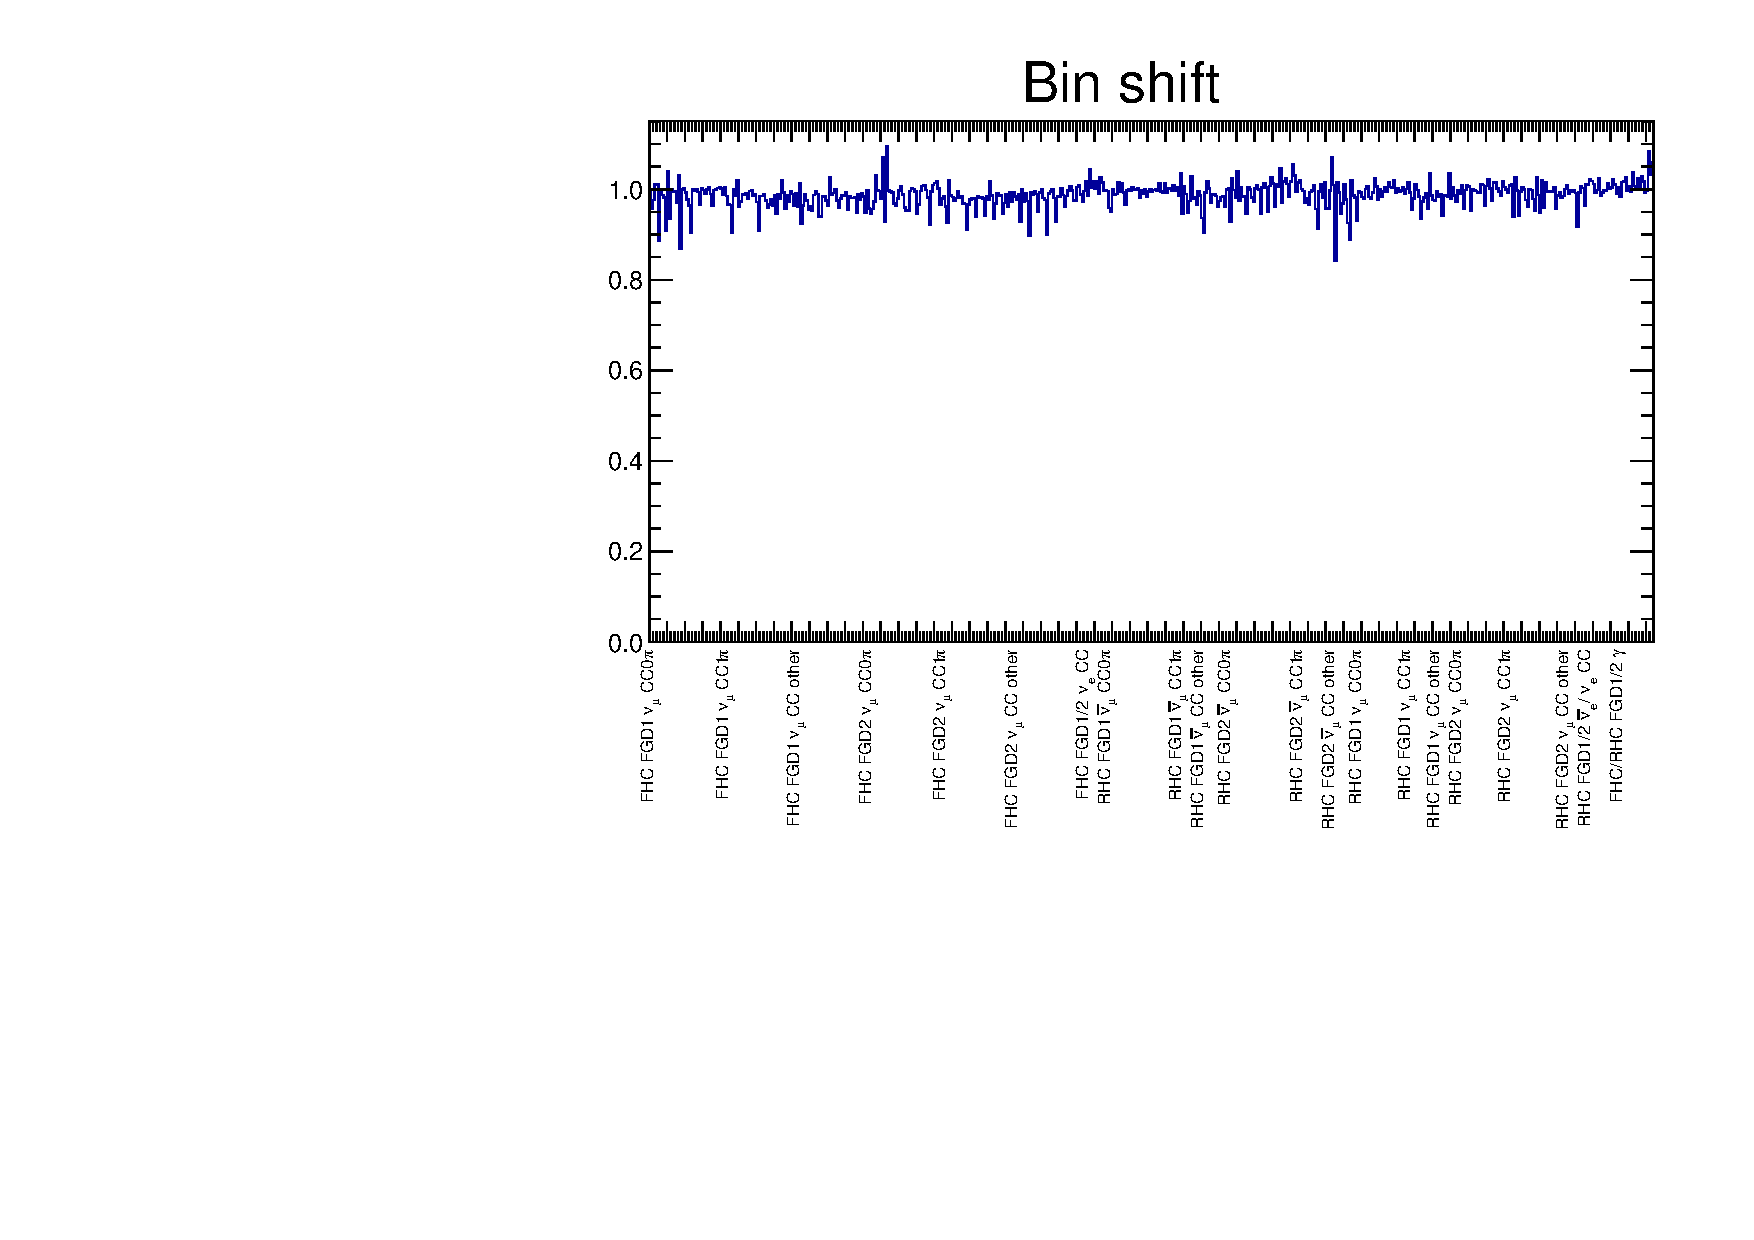
\includegraphics[width=0.78\textwidth]{images/BANFF/Varied_Mean_over_Nominal.pdf} \\
  \caption[Shifts applied to the nominal predictions on the lepton
  reconstructed bins]{Shifts applied to the nominal predictions on the
    lepton reconstructed bins. The samples are organised as mentioned
    in Table~\ref{tab:samples}.}
  \label{fig:totndcovshift}
\end{figure}
\clearpage

\section{Event rates}
\label{sec:eventrates}
In this section, the event rates are compared for data and
\Gls{MC}. This is done in
Tables~\ref{tab:evratefhc}~and~\ref{tab:evratesrhc}, where each
correction from the previous section is applied independently to build
the so-called \Gls{Asimov} data set~\cite{Cowan:2010js}. The
\Gls{Asimov} data set is the ``best guess'' \Gls{MC} prediction given
all the priors: i.e. this data set is created by setting all the
corrections to their most probable value, given all the prior
knowledge from other experiments, beam settings and detector
parameters.

The statistical weight of the electron neutrino samples is very small
compared to that of the muon neutrino samples. This is due to the fact
that the electron (anti-) neutrino fluxes are much smaller compared to
the muon (anti-) neutrino ones.

Note that around half of the electron~/~positrons from the \Gls{nue},
\Gls{anue} and photon samples have momentum below a $200$~MeV
threshold that was introduced. This was done because at low energy
these samples have a very large and dominant photon contamination.

\begin{table}[ht]
  \begin{adjustbox}{center}
    \tabcolsep=0.11cm
    \begin{tabular}{lllllllll}
      \toprule
      \multirow{2}{*}{Sample} & \multirow{2}{*}{Data} & Raw      & \multirow{2}{*}{\Gls{POT}} & \Gls{POT} & \Gls{POT} & \Gls{POT} & \Gls{POT} & \multirow{2}{*}{Prefit} \\
                              &                       & \Gls{MC} &                            & + Flux    & + XSec    & + Det     & + Shift   &  \\
      \midrule
      \multicolumn{9}{l}{\Gls{FHC} \Gls{FGD}1}              \\
      \midrule
      \Gls{numu} \Gls{CC} $0\pi$    &  33548 &  459887 &  31468.27 &  37255.42 &  29993.65 &  30301.11 & 31094.08 & 33889.88\\
      \Gls{numu} \Gls{CC} $1\pi$    &  7755  &  117199 &  8057.27  &  10357.07 &  7580.53  &  7686.00  & 7876.86  & 9136.50 \\
      \Gls{numu} \Gls{CC} other     &  8052  &  90341  &  6208.35  &  8813.59  &  6148.81  &  5902.42  & 6080.17  & 8136.08 \\
      \Gls{nue}  \Gls{CC}           &  297   &  5865   &  326.80   &  421.73   &  319.35   &  312.29   & 329.53   & 398.38  \\
      photon                        &  153   &  3036   &  174.13   &  225.53   &  173.01   &  167.42   & 175.37   & 217.68  \\
      \midrule
      \multicolumn{9}{l}{\Gls{FHC} \Gls{FGD}2}              \\
      \midrule
      \Gls{numu} \Gls{CC} $0\pi$    &  33451 &  460361 &  31203.39 &  36941.06 &  29911.08 &  30349.04 & 30628.44 & 33952.94\\
      \Gls{numu} \Gls{CC} $1\pi$    &  6133  &  93215  &  6295.84  &  8161.10  &  5981.79  &  6114.35  & 6156.31  & 7413.34 \\
      \Gls{numu} \Gls{CC} other     &  7640  &  85621  &  5821.90  &  8265.69  &  5776.64  &  5679.64  & 5713.78  & 7868.08 \\
      \Gls{nue}  \Gls{CC}           &  342   &  5909   &  334.20   &  430.65   &  328.70   &  316.06   & 336.02   & 403.72  \\
      photon                        &  147   &  2810   &  157.09   &  203.99   &  155.63   &  148.12   & 157.87   & 191.86  \\
      \bottomrule
    \end{tabular}
  \end{adjustbox}
  \caption[Event rates at the ND280 for the neutrino mode
  samples]{Event rates at the \Gls{ND} for the neutrino mode samples,
    data (first column). The bare Monte Carlo (Raw \Gls{MC} column)
    was scaled to the data according to the \Gls{POT} (\Gls{POT}
    column), the neutrino flux was reweighted according to the
    NA61~/~SHINE thin target
    measurements~\cite{Abgrall:2011ae,Abgrall:2011ts,Abgrall:2015hmv}
    (\Gls{POT} + Flux column), tuned to external data for the cross
    section shifts~\cite{TN315} (\Gls{POT} + XSec column), all the
    detector parameters were changed according to {\it in situ}
    measurements of cosmic, sand, and through going muons (\Gls{POT} +
    Det) and corrected for non gaussianity of the detector throws
    (\Gls{POT} + Shift). The last column shows the effect of all the
    corrections on the event rates (Prefit column).}
  \label{tab:evratefhc}
\end{table}

\begin{table}[ht]
  \begin{adjustbox}{center}
    \tabcolsep=0.11cm

    \begin{tabular}{lllllllll}
      \toprule
      \multirow{2}{*}{Sample} & \multirow{2}{*}{Data} & Raw      & \multirow{2}{*}{\Gls{POT}} & \Gls{POT} & \Gls{POT} & \Gls{POT} & \Gls{POT} & \multirow{2}{*}{Prefit} \\
                              &                       & \Gls{MC} &                            & + Flux    & + XSec    & + Det     & + Shift   &  \\
      \midrule
      \multicolumn{9}{l}{\Gls{RHC} \Gls{FGD}1}              \\
      \midrule
      \Gls{anumu} \Gls{CC} $0\pi$    &  6367 &  96574 &  6781.46 &  7218.22 &  6229.52 &  6721.28 & 6715.31 & 6497.48\\
      \Gls{anumu} \Gls{CC} $1\pi$    &  535  &  9150  &  640.62  &  686.50  &  541.59  &  624.69  & 635.00  & 562.22 \\
      \Gls{anumu} \Gls{CC} other     &  1070 &  14713 &  1044.25 &  1174.19 &  1001.93 &  1022.28 & 1008.39 & 1076.07\\
      \Gls{numu}  \Gls{CC} $0\pi$    &  2707 &  34939 &  2456.68 &  2866.54 &  2383.68 &  2378.80 & 2448.31 & 2687.39\\
      \Gls{numu}  \Gls{CC} $1\pi$    &  846  &  12344 &  870.87  &  1046.66 &  821.61  &  837.53  & 854.92  & 935.32 \\
      \Gls{numu}  \Gls{CC} other     &  1012 &  10859 &  761.64  &  965.19  &  754.44  &  730.97  & 748.87  & 901.59 \\
      \Gls{anue}  \Gls{CC}           &  79   &  1223  &  86.30   &  86.68   &  81.56   &  88.68   & 87.65   & 86.73  \\
      \Gls{nue}   \Gls{CC}           &  141  &  2010  &  140.97  &  152.31  &  138.88  &  138.28  & 140.98  & 152.79 \\
      photon                         &  83   &  1227  &  88.18   &  98.15   &  88.45   &  85.79   & 88.90   & 96.68  \\
      \midrule
      \multicolumn{9}{l}{\Gls{RHC} \Gls{FGD}2}              \\
      \midrule
      \Gls{anumu} \Gls{CC} $0\pi$    &  6451 & 95543 & 6688.79 &  7124.82 &  6170.68 &  6574.83 & 6681.16 & 6450.17\\
      \Gls{anumu} \Gls{CC} $1\pi$    &  465  & 8160  & 568.38  &  622.08  &  494.13  &  552.79  & 552.55  & 512.04 \\
      \Gls{anumu} \Gls{CC} other     &  1004 & 13443 & 943.85  &  1064.33 &  911.63  &  928.26  & 896.00  & 962.03 \\
      \Gls{numu}  \Gls{CC} $0\pi$    &  2645 & 35130 & 2454.59 &  2861.12 &  2393.86 &  2415.67 & 2447.32 & 2742.4 \\
      \Gls{numu}  \Gls{CC} $1\pi$    &  693  & 9686  & 674.95  &  813.48  &  636.64  &  660.75  & 666.77  & 746.58 \\
      \Gls{numu}  \Gls{CC} other     &  929  & 10330 & 726.14  &  927.55  &  719.98  &  714.40  & 715.88  & 892.49 \\
      \Gls{anue}  \Gls{CC}           &  96   & 1283  & 90.81   &  90.82   &  85.07   &  89.48   & 91.35   & 84.33  \\
      \Gls{nue}   \Gls{CC}           &  148  & 2071  & 147.74  &  167.16  &  146.92  &  142.79  & 148.66  & 162.50 \\
      photon                         &  71   & 1152  & 80.11   &  89.49   &  79.44   &  76.70   & 81.24   & 86.12  \\
      \bottomrule
    \end{tabular}
  \end{adjustbox}
  \caption[Event rates at the ND280 for the anti-neutrino mode
  samples]{Event rates at the \Gls{ND} for the anti-neutrino mode
    samples, data (first column). The bare Monte Carlo (Raw \Gls{MC}
    column) was scaled to the data according to the \Gls{POT}
    (\Gls{POT} column), the neutrino flux was reweighted according to
    the NA61~/~SHINE thin target
    measurements~\cite{Abgrall:2011ae,Abgrall:2011ts,Abgrall:2015hmv}
    (\Gls{POT} + Flux column), tuned to external data for the cross
    section shifts~\cite{TN315} (\Gls{POT} + XSec column), all the
    detector parameters were changed according to {\it in situ}
    measurements of cosmic, sand, and through going muons (\Gls{POT} +
    Det) and corrected for non gaussianity of the detector throws
    (\Gls{POT} + Shift). The last column shows the effect of all the
    corrections on the event rates (Prefit column).}
  \label{tab:evratesrhc}
\end{table}
\clearpage

\section{Asimov fit}
\label{sec:asimov}
The \Gls{Asimov} data set~\cite{Cowan:2010js} is the data set which is
the ``best guess'' for what the data distribution would be. In the
present case, the \Gls{Asimov} data set is the \Gls{MC} set reweighted
with the \Gls{POT} ratio, with the neutrino flux reweighting according
the to the NA61~/~SHINE thin target
measurement~\cite{Abgrall:2011ae,Abgrall:2011ts,Abgrall:2015hmv}, with
the cross section tuned according to external data~\cite{TN315}, with
all the detector shifts and corrected to non-gaussianity for detector
throws.

The fit of the nominal Monte Carlo (\Gls{Asimov}) is shown in
Figure~\ref{fig:asimovxsec} for the cross section parameters;
Figures~\ref{fig:asimovfluxND}~and~\ref{fig:asimovfluxSK} for the
\Gls{ND} and \Gls{SK} flux parameters, respectively (shown with the
binning of the covariance matrix of the flux,
Figure~\ref{fig:fluxsystematics}); and
Figures~\ref{fig:asimovdet1}~and~\ref{fig:asimovdet2} for all the
detector parameters which control the normalisation of each bin.

The Minuit2 minimisation was run on the PPRC cluster at Queen Mary
University using 25~CPU in parallel. It took 113632 steps for the
minimiser to converge and the HESS method was then ran to estimate the
postfit correlations and errors.

For an \Gls{Asimov} fit, it is important to check that the
implementation of all the systematic uncertainties does not create any
bias in the final distributions and values of the parameters, which is
visible in all the figures mentioned in this section: no parameter is
pulled away from its nominal value, indicating that the minimisation
has taken place normally.

These figures are also indicative of the power of the \Gls{ND} in
constraining the oscillation analysis systematic errors. For example,
one can easily see that the flux uncertainty is largely decreased at
\Gls{SK} after the \Gls{ND} fit. Similarly, this is visible for the
cross section parameters.

The focus of this analysis is on the \Gls{nue}, which for the first
time were used in this kind of fits. One can see that the error on the
$\nu_e / \nu_\mu$ ratio is still larger than the $3\%$ that is used
currently in \Gls{TK} oscillation analyses. In this case, it is
$7.6\%$ for the \Gls{nue} and $19.3\%$ for \Gls{anue}. This means that
the theoretical result in~\cite{Day:2012gb} can still not be tested
with the current data at \Gls{TK}.

On Figures~\ref{fig:asimovcorrall}, strong anti-correlations between
the cross section and flux parameters are visible (blue bands off
diagonal). This is expected, since when the flux is increasing, the
cross section should be smaller for a constant number of events. A
zoom of this region is visible in Figure~\ref{fig:asimovcorrzoom}. It
is interesting to see some correlations appear for the first time
between the flux and the cross section parameters related to the
\Gls{nue} events. This correlation reaches $-35.6\%$ for the highest
energy bin of the \Gls{nue} in \Gls{FHC} and the $\nu_e / \nu_\mu$
error.

Finally, the cross section and flux correlation are visible in
Figure~\ref{fig:asimovcorrflux} and \ref{fig:asimovcorrxsec}. Although
this is still marginal, some correlation between electron (anti-)
neutrino and the other cross section parameters are introduced. The
rest of the correlation are due to the muon (anti-) neutrino
samples:
\begin{itemize}[noitemsep,topsep=0pt]
\item The parameters which acts on the $Q^2$ distribution, such as
  $M_a$ and the \Gls{BeRPA}, get correlated.
\item The parameters which control the \Gls{RES} events gets
  correlated ($M_a^{\text{RES}}$, the isoscalar background and
  $C_A^5$).
\item Some additional correlations between the \Gls{RES} parameters
  and \Gls{2p2h} appear due to the \Gls{RES} events present in the
  \Gls{CC} 0 pion samples.
\item Finally, although the \Gls{FSI} parameter get correlated, they
  are not used in the oscillation analyses fit, they will not be
  discussed here.
\end{itemize}

All of the cross section parameter values before and after the
\Gls{Asimov} fit are shown in Table~\ref{tab:postfitxsec} (note that
these are shown with the real data fit result, in the interest of
space).

\begin{figure}[ht]
  \begin{center}
    \includegraphics[width=0.9\textwidth,page=3]{images/BANFF/OutputAsimov_histos.pdf}
    \caption[Cross section uncertainties before and after a fit to the
    Asimov data set of the ND selections]{Cross section uncertainties
      before (red) and after (blue) a fit to the \Gls{Asimov} data set
      of the \Gls{ND} selections.}
    \label{fig:asimovxsec}
  \end{center}
\end{figure}

\begin{figure}[ht]
  \begin{center}
    \begin{adjustbox}{center}
      \begin{tabular}{cc}
        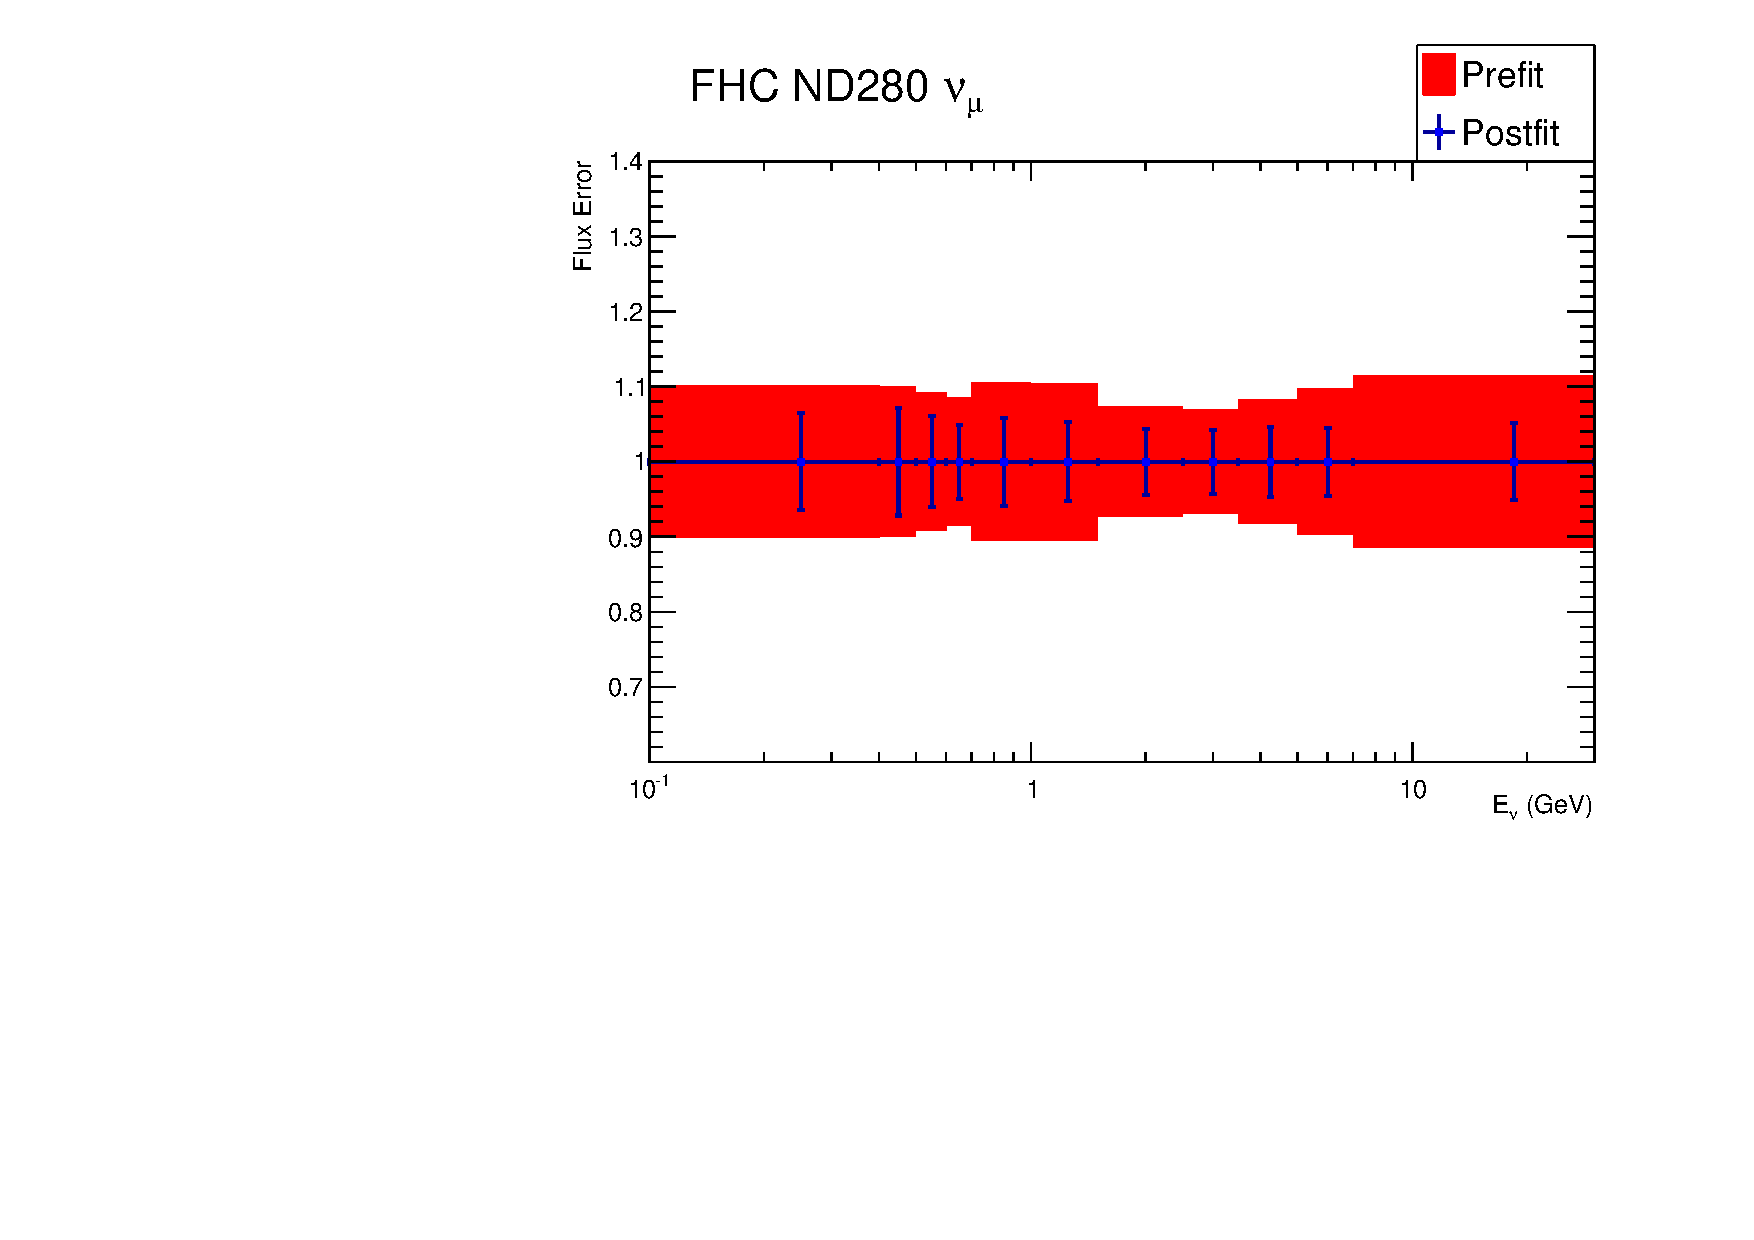
\includegraphics[width=\imagewidth\textwidth,page=1]{images/BANFF/flux_asimov.pdf} & \includegraphics[width=\imagewidth\textwidth,page=2]{images/BANFF/flux_asimov.pdf}\\
        \includegraphics[width=\imagewidth\textwidth,page=3]{images/BANFF/flux_asimov.pdf} & \includegraphics[width=\imagewidth\textwidth,page=4]{images/BANFF/flux_asimov.pdf}\\
        \includegraphics[width=\imagewidth\textwidth,page=5]{images/BANFF/flux_asimov.pdf} & \includegraphics[width=\imagewidth\textwidth,page=6]{images/BANFF/flux_asimov.pdf}\\
        \includegraphics[width=\imagewidth\textwidth,page=7]{images/BANFF/flux_asimov.pdf} & \includegraphics[width=\imagewidth\textwidth,page=8]{images/BANFF/flux_asimov.pdf}\\
      \end{tabular}
    \end{adjustbox}
    \caption[ND280 flux uncertainties before and after a fit to the
    Asimov data set of the ND280 selections]{\Gls{ND} flux
      uncertainties before (red) and after (blue) a fit to the
      \Gls{Asimov} data set of the \Gls{ND} selections.}
    \label{fig:asimovfluxND}
  \end{center}
\end{figure}

\begin{figure}[ht]
  \begin{center}
   \begin{adjustbox}{center}
      \begin{tabular}{cc}
        \includegraphics[width=\imagewidth\textwidth,page=9 ]{images/BANFF/flux_asimov.pdf} & \includegraphics[width=\imagewidth\textwidth,page=10]{images/BANFF/flux_asimov.pdf}\\
        \includegraphics[width=\imagewidth\textwidth,page=11]{images/BANFF/flux_asimov.pdf} & \includegraphics[width=\imagewidth\textwidth,page=12]{images/BANFF/flux_asimov.pdf}\\
        \includegraphics[width=\imagewidth\textwidth,page=13]{images/BANFF/flux_asimov.pdf} & \includegraphics[width=\imagewidth\textwidth,page=14]{images/BANFF/flux_asimov.pdf}\\
        \includegraphics[width=\imagewidth\textwidth,page=15]{images/BANFF/flux_asimov.pdf} & \includegraphics[width=\imagewidth\textwidth,page=16]{images/BANFF/flux_asimov.pdf}\\
      \end{tabular}
    \end{adjustbox}
    \caption[SK flux uncertainties before and after a fit to the
    Asimov data set of the ND280 selections]{\Gls{SK} flux
      uncertainties before (red) and after (blue) a fit to the
      \Gls{Asimov} data set of the \Gls{ND} selections.}
    \label{fig:asimovfluxSK}
  \end{center}
\end{figure}


\begin{figure}[ht]
  \begin{center}
    \includegraphics[width=0.8\textwidth,page=4]{images/BANFF/OutputAsimov_histos.pdf}\\
    \includegraphics[width=0.8\textwidth,page=5]{images/BANFF/OutputAsimov_histos.pdf}
    \caption[ND280 detector and 1p1h uncertainties before and after a
    fit to the Asimov data set of the FHC $\nu_\mu$ ND280
    selections]{\Gls{ND} detector and 1p1h uncertainties before (red)
      and after (blue) a fit over the data from the \Gls{ND}
      selections. The dotted lines are the edges of the
      $\cos(\theta_\text{lepton})$ bins (left to right for increasing
      $\cos(\theta_\text{lepton})$ bins). \textbf{\textit{Top:}}
      \Gls{FHC} \Gls{FGD}1 \Gls{numu} \Gls{CC}
      selections. \textbf{\textit{Bottom:}} \Gls{FHC} \Gls{FGD}2
      \Gls{numu} \Gls{CC} selections.}
    \label{fig:asimovdet1}
  \end{center}
\end{figure}

\begin{figure}[ht]
  \begin{center}
    \includegraphics[width=0.8\textwidth,page=6]{images/BANFF/OutputAsimov_histos.pdf}\\
    \includegraphics[width=0.8\textwidth,page=7]{images/BANFF/OutputAsimov_histos.pdf}
    \caption[ND280 detector and 1p1h uncertainties before and after a
    fit to the Asimov data set of the RHC (anti-)$\nu_\mu$ and
    (anti-)$\nu_e$ ND280 selections]{\Gls{ND} detector and 1p1h
      uncertainties before (red) and after (blue) a fit over the data
      from the \Gls{ND} selections. The dotted lines are the edges of
      the $\cos(\theta_\text{lepton})$ bins (left to right for
      increasing $\cos(\theta_\text{lepton})$
      bins). \textbf{\textit{Top:}} \Gls{RHC} \Gls{FGD}1/2 \Gls{anumu}
      \Gls{CC} selections. \textbf{\textit{Bottom:}} \Gls{RHC}
      \Gls{FGD}1/2 \Gls{numu} \Gls{CC} selections.}
    \label{fig:asimovdet2}
  \end{center}
\end{figure}


\begin{figure}[ht]
  \begin{center}
    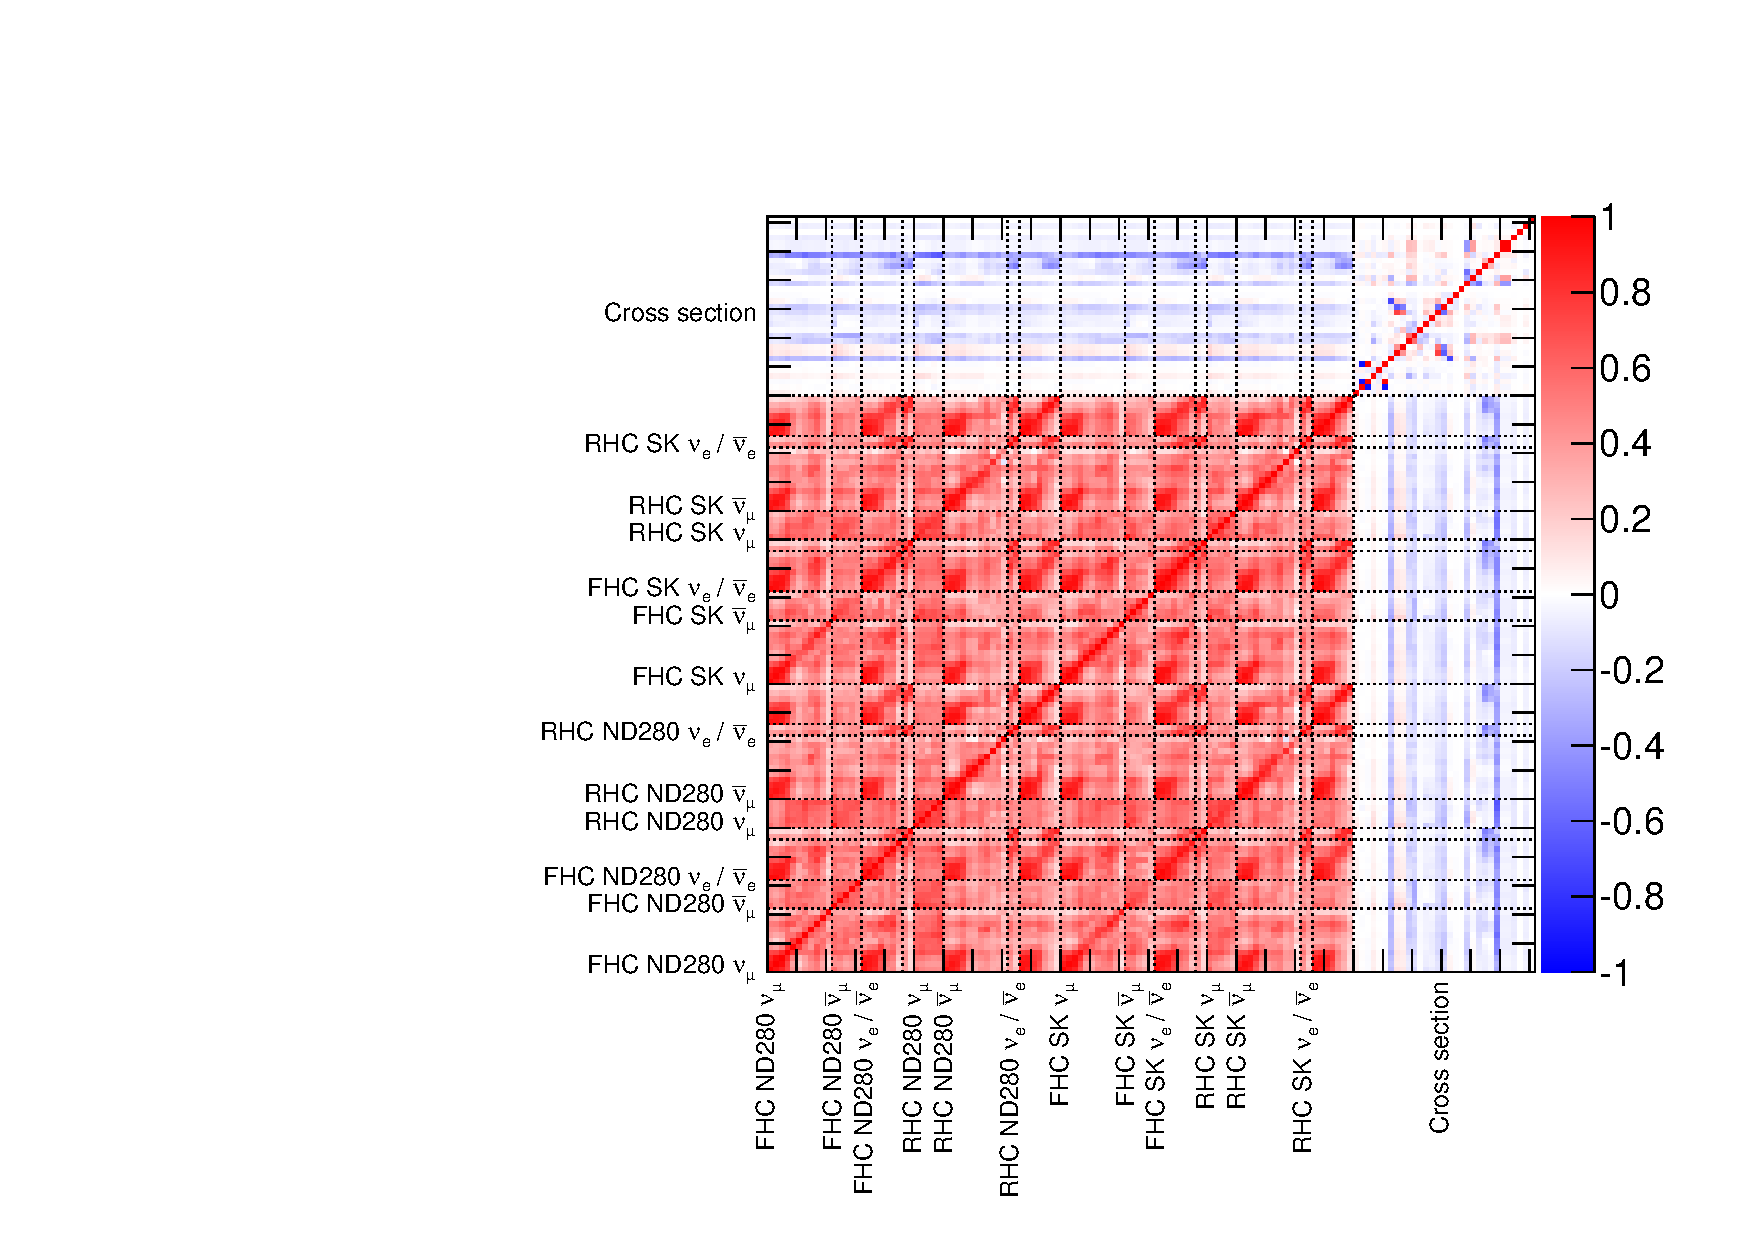
\includegraphics[width=0.9\textwidth,page=1]{images/BANFF/OutputAsimov_matrices.pdf}
    \caption[Correlations between all the parameters used for
    oscillation analyses after a fit to the Asimov data set of the
    ND280 selections]{Correlations between all the parameters used for
      oscillation analyses after a fit to the \Gls{Asimov} data set of
      the \Gls{ND} selections.}
    \label{fig:asimovcorrall}
  \end{center}
\end{figure}

\begin{figure}[ht]
  \begin{center}
    \includegraphics[width=0.9\textwidth,page=5]{images/BANFF/OutputAsimov_matrices.pdf}
    \caption[Correlations between the flux and cross section
    parameters used for oscillation analyses after a fit to the Asimov
    data set of the ND280 selections]{Zoom of
      Figure~\ref{fig:asimovcorrall}, correlations between the flux
      and cross section parameters used for oscillation analyses after
      a fit to the \Gls{Asimov} data set of the \Gls{ND} selections.}
    \label{fig:asimovcorrzoom}
  \end{center}
\end{figure}


\begin{figure}[ht]
  \begin{center}
    \includegraphics[width=0.9\textwidth,page=4]{images/BANFF/OutputAsimov_matrices.pdf}\\
    \caption[Correlation of the flux parameters used for oscillation
    analyses after a fit to the Asimov data set of the ND280
    selection]{Zooms of Figure~\ref{fig:asimovcorrall}, correlation of
      the flux parameters used for oscillation analyses after a fit to
      the \Gls{Asimov} data set of the \Gls{ND}
      selection.}
    \label{fig:asimovcorrflux}
  \end{center}
\end{figure}

\begin{figure}[ht]
  \begin{center}
    \includegraphics[width=0.9\textwidth,page=2]{images/BANFF/OutputAsimov_matrices.pdf}\\
    \caption[Correlation of the cross section parameters used for
    oscillation analyses after a fit to the Asimov data set of the
    ND280 selection]{Zooms of Figure~\ref{fig:asimovcorrall},
      correlation of the cross section parameters used for oscillation
      analyses after a fit to the \Gls{Asimov} data set of the
      \Gls{ND} selection.}
    \label{fig:asimovcorrxsec}
  \end{center}
\end{figure}

\clearpage

\section{Data result}
\label{sec:data}
In this section, the result of the real data fit is commented.
Similarly to what was done for the \Gls{Asimov} fit, the fit was run
using the cluster at Queen Mary University and took 246011 steps to
finalise the minimisation.


\subsection{Data comparisons}
\label{subsec:prefitpostfitdistrib}

\subsubsection{Prefit comparisons}
The one-dimensional muon momentum projections of the \Gls{numu}
selections are shown before and after the data fit in
Figures~\ref{fig:numuCC0Pi}~to~\ref{fig:numubkgCCOth}. Note that all
the corrections listed in the previous sections were applied in the
stacked histograms, they are the ``\Gls{Asimov}'' data sets. On the
bottom of the same figures, the data~/~\Gls{MC} ratios before and
after the fit are shown.

Some interesting features are already visible in the prefit
distributions:
\begin{itemize}[noitemsep,topsep=0pt]
\item In the \Gls{numu} \Gls{CC} 0 pion selections, both in \Gls{FHC}
  and \Gls{RHC} (Figures in~\ref{fig:numuCC0Pi} and
  \ref{fig:numubkgCC0Pi}), the \Gls{MC} distributions are lower than
  the data for low momentum and this is inverted for high energy. This
  could be symptomatic of problems in the form factor at low $Q^2$,
  since most of the high energy events are also very forward, and
  sensitive to the relatively low $Q^2$.
\item In the \Gls{numu} \Gls{CC} 1 pion selections, the \Gls{MC}
  systematically overestimates the data (Figures
  in~\ref{fig:numuCC1Pi} and \ref{fig:anumuCC1Pi}), except in the
  \Gls{RHC} wrong sign component (\Gls{numu}) selections
  (Figure~\ref{fig:numubkgCC1Pi}). There are multiple reasons why this
  could happen. Firstly, the fact that the wrong sign component has a
  different behaviour can mean that the neutrino flux prediction is
  wrong. Secondly, on average the neutrinos in \Gls{RHC} have a higher
  energy. This allow creation of higher mass resonances, for which
  predictions are more complex than for the $\Delta$ resonance.

  The fact that \Gls{anumu} and \Gls{numu} selections (Figures
  in~\ref{fig:numuCC1Pi} and \ref{fig:anumuCC1Pi}) show the same types
  of disagreements does not mean it comes from the same
  mismodelling. There are reasons to believe that the \Gls{RES}
  modelling in anti-neutrino can be significatively wrong, due to the
  more sparse data. Hence, the behaviour of the isoscalar background
  could be different for the case of anti-neutrinos. Finally, since
  the pion is negatively charged for \Gls{anumu} selections, some of
  the \Gls{FSI} parameters such as the charge exchange parameter could
  be very different to the positively charged case.
\item In the \Gls{numu} \Gls{CC} other case, the data is largely
  underestimated at around $1$~GeV, for all the selections (Figures in
  \ref{fig:numuCCother}, \ref{fig:anumuCCOth} and
  \ref{fig:numubkgCCOth}). These selections are sensitive to the
  \Gls{SIS} and \Gls{DIS}, which is probably one of the least well
  simulated part of the \Gls{TK} model due to the absence of reliable
  models. The fact that the data is not reproduced adequatly in these
  regions is not surprising.
\end{itemize}

Next, moving on the \Gls{nue} selections, their one-dimensional
projections are shown from
Figures~\ref{fig:nue}~to~\ref{fig:photonrhc}.  The first observations
of the prefit is that the photon samples are over-estimated (Figures
in~\ref{fig:gamma} and \ref{fig:photonrhc}), this is very similar to
what was observed in the \nisp searches
(Figure~\ref{fig:finalsample}). It also seems that the high momentum
bins of the electron (anti-) neutrino samples are the ones that will
be able to constrain the electron neutrino parameters because they are
purer (Figure in~\ref{fig:nue}, \ref{fig:anue} and \ref{fig:nuebkg}).

In the \Gls{FHC} \Gls{nue} samples (Figures in~\ref{fig:nue}), the
first momentum bin has a data~/~\Gls{MC} disagreement in only the
\Gls{FGD}1 sample: In \Gls{FGD}1 the \Gls{MC} overpredicts the data,
whereas this seems to not be the case for \Gls{FGD}2. This feature is
not visible in the photon control sample (Figures in~\ref{fig:gamma}),
whereas this is marginally visible for \Gls{RHC} samples (\Gls{nue}
and \Gls{anue}, Figures in~\ref{fig:nuebkg} \ref{fig:anue},
respectively). This seem to indicate that there are physical effects
which are not present in the \Gls{MC} for one of the \Gls{FGD}
selections. Given the fact that this is only visible in the electron
(positron) samples and not in the photon sample, such effects are most
likely due to the \Gls{PID} which is realised in
Section~\ref{subsec:electronneutrinoselections}. The difference could
be due to:
\begin{itemize}[noitemsep,topsep=0pt]
\item A difference in the \Gls{TPC}2 and 3 \Gls{PID}, since the photon
  sample uses the invariant mass cut, there is much less dependancy to
  the \Gls{TPC} \Gls{PID} for the photon sample than there is for the
  \Gls{nue} and \Gls{anue} samples.
\item The electron \Gls{ECal} \Gls{PID}, which is, in the case of the
  \Gls{FGD}2 uses the \Gls{DsECal} (see cut described in
  Section~\ref{subsubsec:electronpid}).
\item The second \Gls{TPC} \Gls{PID} cut (see cut described in
  Section~\ref{subsubsec:secondtpcpid}).
\item The usage of the \Gls{FGD}2 shower cut for \Gls{FGD}1 electron
  and positron sample (see cut described in
  Section~\ref{subsubsec:fgd2shower}).
\item The electron
\end{itemize}

Finally, the statistics are quite reduced which
means that the \Gls{ND} is overall not very sensitive to electron
neutrinos.


\subsubsection{Postfit comparisons}
The first thing to notice is that all the data~/~\Gls{MC} ratios get
better for all the samples. These are shown in
Figures~\ref{fig:numuCC0Pi}~to~\ref{fig:photonrhc}. The residual
differences are:
\begin{itemize}[noitemsep,topsep=0pt]
\item In the \Gls{CC} other samples, the data excess still remains
  (Figures in \ref{fig:numuCCother}, \ref{fig:anumuCCOth} and
  \ref{fig:numubkgCCOth}). This probably means that the \Gls{DIS}
  parameter has not enough freedom encoded in it to fit the shape of
  the muon momentum. In fact, the data~/~\Gls{MC} ratios in these
  samples almost do not change, even in the ones that have the highest
  statistical power in neutrino mode.
\item The \Gls{CC} 1 pion samples ratios in \Gls{RHC} (Figures
  in~\ref{fig:anumuCC1Pi} and \ref{fig:numubkgCC1Pi}) almost do not
  change, indicating that the \Gls{FHC} samples are dominating the fit
  to the resonant parameters (Figures in~\ref{fig:numuCC1Pi}). This is
  in general true for most of the \Gls{RHC} samples, it seems that the
  anti-neutrino samples have a reduced impact on the fit due their
  lower statistics, and therefore some adequat anti-neutrino
  parameters need to be designed to let more freedom to the \Gls{MC}
  prediction in these samples.
\item The photon sample low energy discrepancy is not absorbed by the
  fit (Figures in~\ref{fig:gamma} and \ref{fig:photonrhc}), which
  indicates that the photon error has not enough freedom to change the
  shape of the distributions, this means that central values of the
  parameters relevant to \Gls{nue} and \Gls{anue} probably are wrong.
\end{itemize}



\begin{figure}[ht]
  \center
  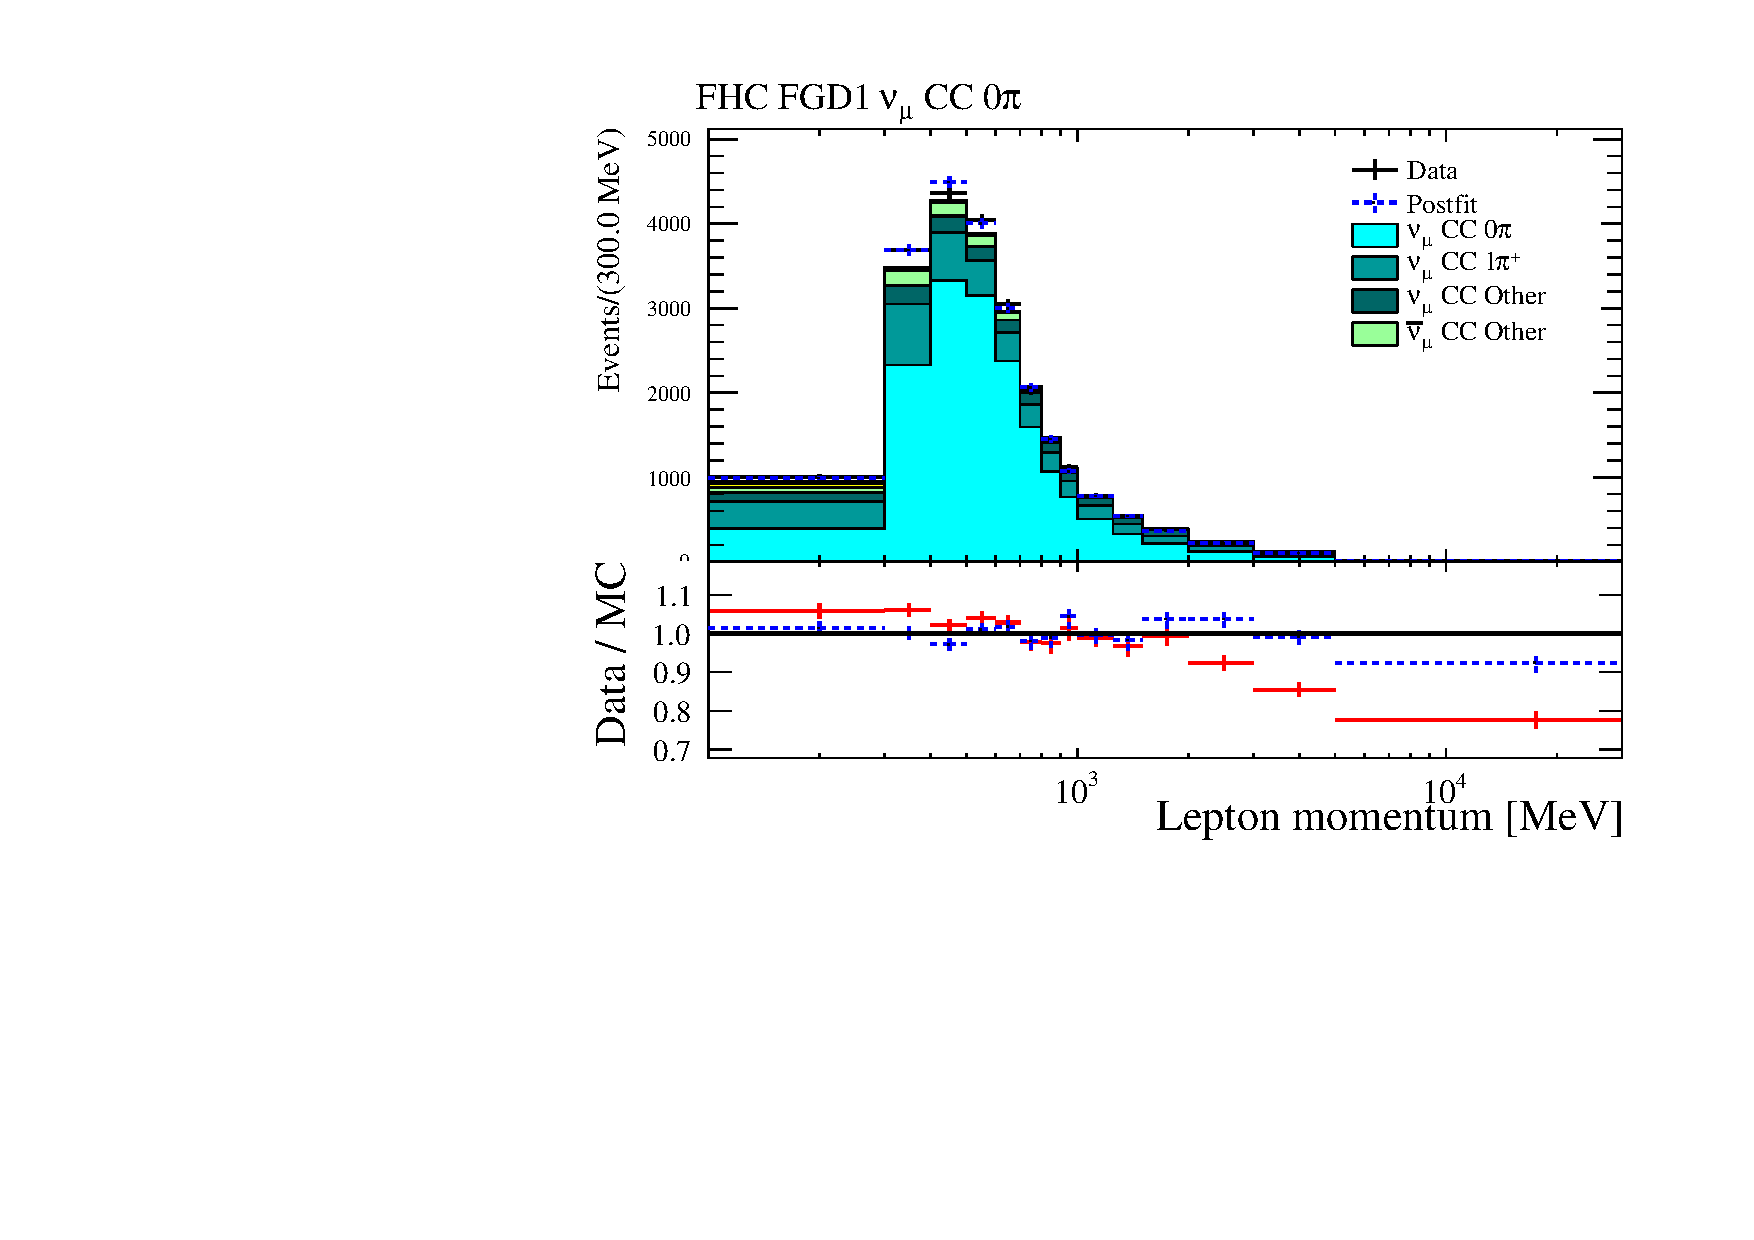
\includegraphics[keepaspectratio=true,width=0.7\textwidth,page=1]{images/BANFF/reactionCodeStacks_PrefitAndPostfit_mom.pdf}\\
  \includegraphics[keepaspectratio=true,width=0.7\textwidth,page=4]{images/BANFF/reactionCodeStacks_PrefitAndPostfit_mom.pdf}\\
  \begin{center}
    \caption[FHC $\nu_\mu$ CC 0 pion FGD1 and 2 samples before and
    after a fit over the data from the ND280
    selections]{One-dimensional projections of the lepton momentum of
      the \Gls{FHC} \Gls{numu} \Gls{CC} 0 pion \Gls{FGD}1 and 2
      samples before (stack) and after (blue dotted) a fit over the
      data from the \Gls{ND} selections. \textbf{\textit{Top:}}
      \Gls{FGD}1. \textbf{\textit{Bottom:}} \Gls{FGD}2. The bottom
      pads on each figure show the data~/~\Gls{MC} ratio before (red)
      and after (blue dotted) the data fit.}
    \label{fig:numuCC0Pi}
  \end{center}
\end{figure}


\begin{figure}[ht]
  \center
  \includegraphics[keepaspectratio=true,width=0.7\textwidth,page=2]{images/BANFF/reactionCodeStacks_PrefitAndPostfit_mom.pdf}\\
  \includegraphics[keepaspectratio=true,width=0.7\textwidth,page=5]{images/BANFF/reactionCodeStacks_PrefitAndPostfit_mom.pdf}\\
  \begin{center}
    \caption[FHC $\nu_\mu$ CC 1 pion FGD1 and 2 samples before and
    after a fit over the data from the ND280
    selections]{One-dimensional projections of the lepton momentum of
      the \Gls{FHC} \Gls{numu} \Gls{CC} 1 pion \Gls{FGD}1 and 2
      samples before (stack) and after (blue dotted) a fit over the
      data from the \Gls{ND} selections. \textbf{\textit{Top:}}
      \Gls{FGD}1. \textbf{\textit{Bottom:}} \Gls{FGD}2. The bottom
      pads on each figure show the data~/~\Gls{MC} ratio before (red)
      and after (blue dotted) the data fit.}
    \label{fig:numuCC1Pi}
  \end{center}
\end{figure}


\begin{figure}[ht]
  \center
  \includegraphics[keepaspectratio=true,width=0.7\textwidth,page=3]{images/BANFF/reactionCodeStacks_PrefitAndPostfit_mom.pdf}\\
  \includegraphics[keepaspectratio=true,width=0.7\textwidth,page=6]{images/BANFF/reactionCodeStacks_PrefitAndPostfit_mom.pdf}\\
  \begin{center}
    \caption[FHC $\nu_\mu$ CC other FGD1 and 2 samples before and
    after a fit over the data from the ND280
    selections]{One-dimensional projections of the lepton momentum of
      the \Gls{FHC} \Gls{numu} \Gls{CC} other \Gls{FGD}1 and 2 samples
      before (stack) and after (blue dotted) a fit over the data from
      the \Gls{ND} selections. \textbf{\textit{Top:}}
      \Gls{FGD}1. \textbf{\textit{Bottom:}} \Gls{FGD}2. The bottom
      pads on each figure show the data~/~\Gls{MC} ratio before (red)
      and after (blue dotted) the data fit.}
    \label{fig:numuCCother}
  \end{center}
\end{figure}


\begin{figure}[ht]
  \center
  \includegraphics[keepaspectratio=true,width=0.7\textwidth,page=7]{images/BANFF/reactionCodeStacks_PrefitAndPostfit_mom.pdf}\\
  \includegraphics[keepaspectratio=true,width=0.7\textwidth,page=10]{images/BANFF/reactionCodeStacks_PrefitAndPostfit_mom.pdf}\\
  \begin{center}
    \caption[RHC $\bar{\nu}_\mu$ CC 0 pion FGD1 and 2 samples before
    and after a fit over the data from the ND280
    selections]{One-dimensional projections of the lepton momentum of
      the \Gls{RHC} \Gls{anumu} \Gls{CC} 0 pion \Gls{FGD}1 and 2
      samples before (stack) and after (blue dotted) a fit over the
      data from the \Gls{ND} selections. \textbf{\textit{Top:}}
      \Gls{FGD}1. \textbf{\textit{Bottom:}} \Gls{FGD}2. The bottom
      pads on each figure show the data~/~\Gls{MC} ratio before (red)
      and after (blue dotted) the data fit.}
    \label{fig:anumuCC0Pi}
  \end{center}
\end{figure}


\begin{figure}[ht]
  \center
  \includegraphics[keepaspectratio=true,width=0.7\textwidth,page=8]{images/BANFF/reactionCodeStacks_PrefitAndPostfit_mom.pdf}\\
  \includegraphics[keepaspectratio=true,width=0.7\textwidth,page=11]{images/BANFF/reactionCodeStacks_PrefitAndPostfit_mom.pdf}\\
  \begin{center}
    \caption[RHC $\bar{\nu}_\mu$ CC 1 pion FGD1 and 2 samples before
    and after a fit over the data from the ND280
    selections]{One-dimensional projections of the lepton momentum of
      the \Gls{RHC} \Gls{anumu} \Gls{CC} 1 pion \Gls{FGD}1 and 2
      samples before (stack) and after (blue dotted) a fit over the
      data from the \Gls{ND} selections. \textbf{\textit{Top:}}
      \Gls{FGD}1. \textbf{\textit{Bottom:}} \Gls{FGD}2. The bottom
      pads on each figure show the data~/~\Gls{MC} ratio before (red)
      and after (blue dotted) the data fit.}
    \label{fig:anumuCC1Pi}
  \end{center}
\end{figure}

\begin{figure}[ht]
  \center
  \includegraphics[keepaspectratio=true,width=0.7\textwidth,page=9]{images/BANFF/reactionCodeStacks_PrefitAndPostfit_mom.pdf}\\
  \includegraphics[keepaspectratio=true,width=0.7\textwidth,page=12]{images/BANFF/reactionCodeStacks_PrefitAndPostfit_mom.pdf}\\
  \begin{center}
    \caption[RHC $\bar{\nu}_\mu$ CC other FGD1 and 2 samples before
    and after a fit over the data from the ND280
    selections]{One-dimensional projections of the lepton momentum of
      the \Gls{RHC} \Gls{anumu} \Gls{CC} other \Gls{FGD}1 and 2
      samples before (stack) and after (blue dotted) a fit over the
      data from the \Gls{ND} selections. \textbf{\textit{Top:}}
      \Gls{FGD}1. \textbf{\textit{Bottom:}} \Gls{FGD}2. The bottom
      pads on each figure show the data~/~\Gls{MC} ratio before (red)
      and after (blue dotted) the data fit.}
    \label{fig:anumuCCOth}
  \end{center}
\end{figure}


\begin{figure}[ht]
  \center
  \includegraphics[keepaspectratio=true,width=0.7\textwidth,page=13]{images/BANFF/reactionCodeStacks_PrefitAndPostfit_mom.pdf} \\
  \includegraphics[keepaspectratio=true,width=0.7\textwidth,page=16]{images/BANFF/reactionCodeStacks_PrefitAndPostfit_mom.pdf} \\
  \begin{center}
    \caption[RHC $\nu_\mu$ CC 0 pion FGD1 and 2 samples before and
    after a fit over the data from the ND280
    selections]{One-dimensional projections of the lepton momentum of
      the \Gls{RHC} \Gls{numu} \Gls{CC} 0 pion \Gls{FGD}1 and 2
      samples before (stack) and after (blue dotted) a fit over the
      data from the \Gls{ND} selections. \textbf{\textit{Top:}}
      \Gls{FGD}1. \textbf{\textit{Bottom:}} \Gls{FGD}2. The bottom
      pads on each figure show the data~/~\Gls{MC} ratio before (red)
      and after (blue dotted) the data fit.}
    \label{fig:numubkgCC0Pi}
  \end{center}
\end{figure}


\begin{figure}[ht]
  \center
  \includegraphics[keepaspectratio=true,width=0.7\textwidth,page=14]{images/BANFF/reactionCodeStacks_PrefitAndPostfit_mom.pdf}\\
  \includegraphics[keepaspectratio=true,width=0.7\textwidth,page=17]{images/BANFF/reactionCodeStacks_PrefitAndPostfit_mom.pdf}\\
  \begin{center}
    \caption[RHC $\nu_\mu$ CC 1 pion FGD1 and 2 samples before and
    after a fit over the data from the ND280
    selections]{One-dimensional projections of the lepton momentum of
      the \Gls{RHC} \Gls{numu} \Gls{CC} 1 pion \Gls{FGD}1 and 2
      samples before (stack) and after (blue dotted) a fit over the
      data from the \Gls{ND} selections. \textbf{\textit{Top:}}
      \Gls{FGD}1. \textbf{\textit{Bottom:}} \Gls{FGD}2. The bottom
      pads on each figure show the data~/~\Gls{MC} ratio before (red)
      and after (blue dotted) the data fit.}
    \label{fig:numubkgCC1Pi}
  \end{center}
\end{figure}

\begin{figure}[ht]
  \center
  \includegraphics[keepaspectratio=true,width=0.7\textwidth,page=15]{images/BANFF/reactionCodeStacks_PrefitAndPostfit_mom.pdf}\\
  \includegraphics[keepaspectratio=true,width=0.7\textwidth,page=18]{images/BANFF/reactionCodeStacks_PrefitAndPostfit_mom.pdf}\\
  \begin{center}
    \caption[RHC $\nu_\mu$ CC other FGD1 and 2 samples before and
    after a fit over the data from the ND280
    selections]{One-dimensional projections of the lepton momentum of
      the \Gls{RHC} \Gls{numu} \Gls{CC} other \Gls{FGD}1 and 2 samples
      before (stack) and after (blue dotted) a fit over the data from
      the \Gls{ND} selections. \textbf{\textit{Top:}}
      \Gls{FGD}1. \textbf{\textit{Bottom:}} \Gls{FGD}2. The bottom
      pads on each figure show the data~/~\Gls{MC} ratio before (red)
      and after (blue dotted) the data fit.}
    \label{fig:numubkgCCOth}
  \end{center}
\end{figure}


\begin{figure}[ht]
  \center
  \includegraphics[keepaspectratio=true,width=0.7\textwidth,page=19]{images/BANFF/reactionCodeStacks_PrefitAndPostfit_mom.pdf}\\
  \includegraphics[keepaspectratio=true,width=0.7\textwidth,page=20]{images/BANFF/reactionCodeStacks_PrefitAndPostfit_mom.pdf}\\
  \begin{center}
    \caption[FHC $\nu_e$ CC FGD1 and 2 samples before and after a fit
    over the data from the ND280 selections]{One-dimensional
      projections of the lepton momentum of the \Gls{FHC} \Gls{nue}
      \Gls{CC} inclusive \Gls{FGD}1 and 2 samples before (stack) and
      after (blue dotted) a fit over the data from the \Gls{ND}
      selections. \textbf{\textit{Top:}}
      \Gls{FGD}1. \textbf{\textit{Bottom:}} \Gls{FGD}2. The bottom
      pads on each figure show the data~/~\Gls{MC} ratio before (red)
      and after (blue dotted) the data fit.}
    \label{fig:nue}
  \end{center}
\end{figure}

\begin{figure}[ht]
  \center
  \includegraphics[keepaspectratio=true,width=0.7\textwidth,page=25]{images/BANFF/reactionCodeStacks_PrefitAndPostfit_mom.pdf}\\
  \includegraphics[keepaspectratio=true,width=0.7\textwidth,page=26]{images/BANFF/reactionCodeStacks_PrefitAndPostfit_mom.pdf}
  \begin{center}
    \caption[FHC photon FGD1 and 2 samples before and after a fit over
    the data from the ND280 selections]{One-dimensional projections of
      the lepton momentum of the \Gls{FHC} photon \Gls{FGD}1 and 2
      samples before (stack) and after (blue dotted) a fit over the
      data from the \Gls{ND} selections. \textbf{\textit{Top:}}
      \Gls{FGD}1. \textbf{\textit{Bottom:}} \Gls{FGD}2. The bottom
      pads on each figure show the data~/~\Gls{MC} ratio before (red)
      and after (blue dotted) the data fit.}
    \label{fig:gamma}
  \end{center}
\end{figure}


\begin{figure}[ht]
  \center
  \includegraphics[keepaspectratio=true,width=0.7\textwidth,page=21]{images/BANFF/reactionCodeStacks_PrefitAndPostfit_mom.pdf}\\
  \includegraphics[keepaspectratio=true,width=0.7\textwidth,page=22]{images/BANFF/reactionCodeStacks_PrefitAndPostfit_mom.pdf}
  \begin{center}
    \caption[RHC $\bar{\nu}_e$ FGD1 and 2 samples before and after a
    fit over the data from the ND280 selections]{One-dimensional
      projections of the lepton momentum of the \Gls{RHC} \Gls{anue}
      \Gls{CC} inclusive \Gls{FGD}1 and 2 samples before (stack) and
      after (blue dotted) a fit over the data from the \Gls{ND}
      selections. \textbf{\textit{Top:}}
      \Gls{FGD}1. \textbf{\textit{Bottom:}} \Gls{FGD}2. The bottom
      pads on each figure show the data~/~\Gls{MC} ratio before (red)
      and after (blue dotted) the data fit.}
    \label{fig:anue}
  \end{center}
\end{figure}


\begin{figure}[ht]
  \center
  \includegraphics[keepaspectratio=true,width=0.7\textwidth,page=23]{images/BANFF/reactionCodeStacks_PrefitAndPostfit_mom.pdf}\\
  \includegraphics[keepaspectratio=true,width=0.7\textwidth,page=24]{images/BANFF/reactionCodeStacks_PrefitAndPostfit_mom.pdf}\\
  \begin{center}
    \caption[RHC $\nu_e$ FGD1 and 2 samples before and after a fit
    over the data from the ND selections]{One-dimensional projections
      of the lepton momentum of the \Gls{RHC} \Gls{nue} \Gls{CC}
      inclusive \Gls{FGD}1 and 2 samples before (stack) and after
      (blue dotted) a fit over the data from the \Gls{ND}
      selections. \textbf{\textit{Top:}}
      \Gls{FGD}1. \textbf{\textit{Bottom:}} \Gls{FGD}2. The bottom
      pads on each figure show the data~/~\Gls{MC} ratio before (red)
      and after (blue dotted) the data fit.}
    \label{fig:nuebkg}
  \end{center}
\end{figure}


\begin{figure}[ht]
  \center
  \includegraphics[keepaspectratio=true,width=0.7\textwidth,page=27]{images/BANFF/reactionCodeStacks_PrefitAndPostfit_mom.pdf}\\
  \includegraphics[keepaspectratio=true,width=0.7\textwidth,page=28]{images/BANFF/reactionCodeStacks_PrefitAndPostfit_mom.pdf}\\
  \begin{center}
    \caption[RHC photon FGD1 and 2 samples before and after a fit over
    the data from the ND280 selections]{One-dimensional projections of
      the lepton momentum of the \Gls{RHC} photon \Gls{FGD}1 and 2
      samples before (stack) and after (blue dotted) a fit over the
      data from the \Gls{ND} selections. \textbf{\textit{Top:}}
      \Gls{FGD}1. \textbf{\textit{Bottom:}} \Gls{FGD}2. The bottom
      pads on each figure show the data~/~\Gls{MC} ratio before (red)
      and after (blue dotted) the data fit.}
    \label{fig:photonrhc}
  \end{center}
\end{figure}
\clearpage

\subsection{Fitted systematic uncertainties}
\label{subsec:fittedoscillationsystematics}

For the parameters after the data fit, it should be first noted in
Figure~\ref{fig:dataflux} that there is an overall decrease in the
flux. The flux is very correlated, therefore it is not very surprising
to see group effects of this sort. Note that the high energy
\Gls{anue} parameter, (the only parameter in Figure~\ref{fig:dataflux}
which is pulled higher than its prefit value), is predominantly
governed by the kaon flux, which is somewhat decorrelated from the
bulk of the flux (which comes from pion and muon).

\begin{figure}[ht]
  \begin{center}
    \begin{adjustbox}{center}
      \begin{tabular}{cc}
        \includegraphics[width=0.6\textwidth,page=1]{images/BANFF/OutputData_histos.pdf}\\
        \includegraphics[width=0.6\textwidth,page=2]{images/BANFF/OutputData_histos.pdf}
      \end{tabular}
    \end{adjustbox}
    \caption[Flux uncertainties before and after a fit over the data
    from the ND280 selections]{Flux uncertainties before (red) and
      after (blue) a fit over the data from the \Gls{ND}
      selections. \textbf{\textit{Top:}} \Gls{ND}
      flux. \textbf{\textit{Bottom:}} \Gls{SK} flux.}
    \label{fig:dataflux}
  \end{center}
\end{figure}



Other interesting features can be seen in the
Figure~\ref{fig:dataxsec} and
Table~\ref{tab:postfitxsec}\footnote{Note that the equivalent table
  for the flux can be found in Apprendix~\ref{app:fluxparam}}, which
show the value of the fitted cross section parameters. The most
important is the \Gls{2p2h}-shape for carbon which reaches the limit
of its allowed value (which should be in the range 0 to 2). This is
not a new feature~\cite{TN324} and was already observed for previous
fits which were not using the \Gls{nue} samples and and the
multi-track samples in \Gls{RHC}, unlike the previous time this is
only visible for the carbon parameter. Previously, this behaviour had
been seen for the oxygen counterpart as well. The \Gls{2p2h}
normalisation is also pulled away from its prefit value in the case of
anti-neutrino. This considered as acceptable since the ratio of
normalisation between \Gls{2p2h} neutrinos and anti-neutrinos is not
well known, which differs between
models~\cite{MartiniNpNh1,MartiniNpNh2,NievesNpNh1,NievesNpNh2}.

Although within their acceptable prefit errors, it seems that the
Fermi momentum parameters are also reaching their lower limit values
($186\text{~MeV}$ and $194\text{~MeV}$ for carbon and oxygen,
respectively).

The addition of data corresponding to the run~8 for the \Gls{numu}
selections is confirming that there is a major deficiency of our
modelling for these cross sections. Similarly, the BeRPA$_B$ gets
pulled far away from its prior value. This, again, highlights that the
$Q^2$ parametrisation that is used cannot reproduce the observed data.

The \Gls{nue} and \Gls{anue} parameters are pulled away from the
nominal value, however they have at this stage a too large uncertainty
to claim a mismodelling in this sector.

The isoscalar background parameter is also pulled away, which is due
to the addition of samples more sensitive to anti-neutrino, however
this is also not a new feature of the data~\cite{TN324}.

Finally, the only other parameter which is pulled away from its
nominal value is the \Gls{DIS} parameter. Again this is not new, but
the effect is increased by the fact that the selections are more
sensitive than before to a mismodelling in the \Gls{DIS} sector
because the \Gls{RHC} selections are now using the multi-pion
selections, and the increase in the statistical power due to the
addition of the run~8 data.


\begin{figure}[ht]
  \begin{center}
    \includegraphics[width=0.9\textwidth,page=3]{images/BANFF/OutputData_histos.pdf}
    \caption[Cross section uncertainties before and after a fit over
    the data from the ND280 selections]{Cross section uncertainties
      before (red) and after (blue) a fit over the data from the
      \Gls{ND} selections.}
    \label{fig:dataxsec}
  \end{center}
\end{figure}

\begin{table}[ht]
  \center
  \begin{tabular}{llll}
    \toprule
    Parameter & Prefit & \Gls{Asimov} fit & Data fit  \\
    \midrule
    $M_a^{\text{QE}}$(GeV/c$^2$)           & 1.2              & 1.2 $\pm$ 0.063 & 1.09 $\pm$ 0.07     \\ 
    $p_F^C$(MeV/c)                       & 217.0            & 217.0 $\pm$ 25  & 200.0 $\pm$ 0.02    \\ 
    $p_F^O$(MeV/c)                       & 225.0            & 225.0 $\pm$ 35  & 200.0 $\pm$ 0.04    \\ 
    \gls{2p2h} normalisation $\nu$       & 1.0 $\pm$ 1.0    & 1.0 $\pm$ 0.19  & 1.03 $\pm$ 0.17     \\ 
    \gls{2p2h} normalisation $\bar{\nu}$ & 1.0 $\pm$ 1.0    & 1.0 $\pm$ 0.3   & 0.69 $\pm$ 0.17     \\ 
    \gls{2p2h} normalisation C to O      & 1.0 $\pm$ 0.2    & 1.0 $\pm$ 0.18  & 0.99 $\pm$ 0.18     \\ 
    \gls{2p2h} shape C                   & 100 $\pm$ 300    & 100 $\pm$ 33  & 200 $\pm$ 0.5         \\ 
    \gls{2p2h} shape O                   & 100 $\pm$ 300    & 100 $\pm$ 57  & 103 $\pm$ 29          \\ 
    BeRPA$_A$                            & 0.59 $\pm$ 0.12  & 0.59 $\pm$ 0.08 & 0.63 $\pm$ 0.04     \\ 
    BeRPA$_B$                            & 1.1 $\pm$ 0.2    & 1.05 $\pm$ 0.10 & 1.71 $\pm$ 0.11     \\ 
    BeRPA$_D$                            & 1.13 $\pm$ 0.17  & 1.13 $\pm$ 0.11 & 0.92 $\pm$ 0.13     \\ 
    BeRPA$_E$                            & 0.9 $\pm$ 0.4    & 0.88 $\pm$ 0.35 & 0.8 $\pm$ 0.4       \\ 
    BeRPA$_U$                            & 1.2 $\pm$ 0.1    & 1.2 $\pm$ 0.1   & 1.2 $\pm$ 0.1       \\ 
    $C_a^5$                              & 0.96 $\pm$ 0.15  & 0.96 $\pm$ 0.06 & 0.95 $\pm$ 0.05     \\ 
    $M_a^{\text{RES}}$(GeV/c$^2$)          & 1.07 $\pm$ 0.15  & 1.07 $\pm$ 0.04 & 0.81 $\pm$ 0.04     \\ 
    Isoscalar Background                 & 0.96 $\pm$ 0.4   & 0.96 $\pm$ 0.3  & 1.7 $\pm$ 0.2       \\ 
    $\nu_e/\nu_\mu$                       & 1.0 $\pm$ 1.4  & 1.0 $\pm$ 0.08  & 0.82 $\pm$ 0.07       \\ 
    $\bar{\nu}_e/\bar{\nu}_\mu$           & 1.0 $\pm$ 1.4  & 1.0 $\pm$ 0.19  & 1.1 $\pm$ 0.2         \\ 
    \Gls{CC} \Gls{DIS}                   & 0.0 $\pm$ 0.4    & 0.0 $\pm$ 0.17  & 0.9 $\pm$ 0.2       \\ 
    \Gls{CC} \Gls{COH} C                 & 1.0 $\pm$ 0.3    & 1.0 $\pm$ 0.2   & 1.0 $\pm$ 0.2       \\ 
    \Gls{CC} \Gls{COH} O                 & 1.0 $\pm$ 0.3    & 1.0 $\pm$ 0.2   & 1.0 $\pm$ 0.2       \\ 
    \Gls{NC} \Gls{COH}                   & 1.0 $\pm$ 0.3    & 1.0 $\pm$ 0.3   & 0.7 $\pm$ 0.3       \\ 
    \Gls{NCg}                            & 1.0 $\pm$ 1.0    & 1.0 $\pm$ 1.0   & 1.0 $\pm$ 1.0       \\ 
    other \Gls{NC} at \Gls{ND}           & 1.0 $\pm$ 0.3    & 1.0 $\pm$ 0.2   & 1.3 $\pm$ 0.2       \\ 
    other \Gls{NC} at \Gls{SK}           & 1.0 $\pm$ 0.3    & 1.0 $\pm$ 0.3   & 1.0 $\pm$ 0.3       \\
    \Gls{FSI} Inelastic LowE             & 0.0 $\pm$ 0.4    & 0.0 $\pm$ 0.13  & -0.18 $\pm$ 0.14    \\
    \Gls{FSI} Inelastic HighE            & 0.0 $\pm$ 0.3    & 0.0 $\pm$ 0.16  & -0.11 $\pm$ 0.13    \\ 
    \Gls{FSI} $\pi$ production           & 0.0 $\pm$ 0.5    & 0.0 $\pm$ 0.23  & 0.14 $\pm$ 0.19     \\ 
    \Gls{FSI} $\pi$ absorption           & 0.0 $\pm$ 0.4    & 0.0 $\pm$ 0.18  & 0.13 $\pm$ 0.16     \\ 
    \Gls{FSI} Charge exchange LowE       & 0.0 $\pm$ 0.6    & 0.0 $\pm$ 0.3   & 0.2 $\pm$ 0.3       \\ 
    \Gls{FSI} Charge exchange HighE      & 0.0 $\pm$ 0.3    & 0.0 $\pm$ 0.13  & 0.08 $\pm$ 0.10     \\ 
    \bottomrule
  \end{tabular}
  \caption{Cross section parameters values and uncertainties before
    and after an \Gls{Asimov} fit and a data fit.}
  \label{tab:postfitxsec}
\end{table}
\clearpage

Figures~\ref{fig:datadet1} and \ref{fig:datadet2} shows an interesting feature. At high angle
in the \Gls{CC}0 pion sector, the detector and 1p1h parameters are
pulled to low value (indicating that the \Gls{MC} was overpredicting
the data) and this tendancy is inverted at high momentum. This
probably indicates a problem in the 1p1h error, however the fact that
these parameters affect directly the bin normalisation of the bin, it
is hard to draw any conclusion. However, since this is the part of the
model that is not propagated, this is somehow a smaller
problem. Similar features have been observed previously~\cite{TN324}.

\begin{figure}[ht]
  \begin{center}
    \includegraphics[width=0.8\textwidth,page=6]{images/BANFF/OutputData_histos.pdf}\\
    \includegraphics[width=0.8\textwidth,page=7]{images/BANFF/OutputData_histos.pdf}
    \caption[ND280 detector and 1p1h uncertainties before and after a
    fit over the data from the FHC $\nu_\mu$ ND280
    selections]{\Gls{ND} detector and 1p1h uncertainties before (red)
      and after (blue) a fit over the data from the \Gls{ND}
      selections. The dotted lines are the edges of the
      $\cos(\theta_\text{lepton})$ bins (left to right for increasing
      $\cos(\theta_\text{lepton})$ bins). \textbf{\textit{Top:}}
      \Gls{FHC} \Gls{FGD}1 \Gls{numu} \Gls{CC} selections.
      \textbf{\textit{Bottom:}} \Gls{FHC} \Gls{FGD}2 \Gls{numu}
      \Gls{CC} selections.}
    \label{fig:datadet1}
  \end{center}
\end{figure}

\begin{figure}[ht]
  \begin{center}
    \includegraphics[width=0.8\textwidth,page=6]{images/BANFF/OutputData_histos.pdf}\\
    \includegraphics[width=0.8\textwidth,page=7]{images/BANFF/OutputData_histos.pdf}
    \caption[ND280 detector and 1p1h uncertainties before and after a
    fit over the data from the RHC (anti-)$\nu_\mu$ and
    (anti-)$\nu_e$ND280 selections]{\Gls{ND} detector and 1p1h
      uncertainties before (red) and after (blue) a fit over the data
      from the \Gls{ND} selections. The dotted lines are the edges of
      the $\cos(\theta_\text{lepton})$ bins (left to right for
      increasing $\cos(\theta_\text{lepton})$
      bins). \textbf{\textit{Top:}} \Gls{RHC} \Gls{FGD}1/2 \Gls{anumu}
      \Gls{CC} selections.  \textbf{\textit{Bottom:}} \Gls{RHC}
      \Gls{FGD}1/2 \Gls{numu} \Gls{CC} selections.}
    \label{fig:datadet2}
  \end{center}
\end{figure}
\clearpage

The top of Figure~\ref{fig:datacorrxsec} and the strong
anti-correlation between the \Gls{BeRPA}$_D$ parameter and the axial
mass ($M_a^{QE}$) indicate an unexpected behaviour at high $Q^2$ for
the \Gls{CCQE} events. This could either be related to the \Gls{2p2h}
parametrisation (for example if it does not fill some regions of the
parameter space, then the \Gls{BeRPA} parameters could be used to fill
the missing events), or, alternatively, this could relate to problem
in the \Gls{CCQE} form factor (it could be that the dipole
parametrisation, in Equation~(\ref{eq:ccqeff}), is not an appropriate
choice).

In any case, it is very likely that a $p_\text{value}$ calculation
(after throwing toy experiments) would be very low, however the fit
seems to perform better than the ones used for previous
analyses~\cite{TN324}, with clearer but localised deficiencies in the
models. This is due to the better statistics and to the better
discriminating power in \Gls{RHC} with the multi-pion samples.

\begin{figure}[ht]
  \begin{center}
    \includegraphics[width=0.9\textwidth,page=4]{images/BANFF/OutputData_matrices.pdf}
    \caption[Correlation of the flux parameters used for oscillation
    analyses after a fit to the data of the ND280 selection]{Zoom of
      Figure~\ref{fig:asimovcorrall}, correlation of the flux
      parameters used for oscillation analyses after a fit to the data
      of the \Gls{ND} selection.}
    \label{fig:datacorrflux}
  \end{center}
\end{figure}

\begin{figure}[ht]
  \begin{center}
    \includegraphics[width=0.9\textwidth,page=2]{images/BANFF/OutputData_matrices.pdf}\\
    \caption[Correlation of the cross section parameters used for
    oscillation analyses after a fit to the data of the ND280
    selection]{Zoom of Figure~\ref{fig:asimovcorrall}, correlation of
      the cross section parameters used for oscillation analyses after
      a fit to the data of the \Gls{ND} selection.}
    \label{fig:datacorrxsec}
  \end{center}
\end{figure}

\clearpage
\section{Discussion and future}
\label{sec:discussion}
In this section, the errors in the \Gls{Asimov} fit described in
Section~\ref{sec:asimov} are propagated to the following \Gls{SK}
\Gls{Asimov} data set:
\begin{itemize}[noitemsep,topsep=0pt]
\item \Gls{FHC} muon one ring,
\item \Gls{RHC} muon one ring,
\item \Gls{FHC} electron one ring,
\item \Gls{RHC} electron one ring,
\item \Gls{RHC} electron one ring + one Michel electron.
\end{itemize}
These samples are sensitive to oscillation parameters, so to construct
this \Gls{Asimov} data sets, the values in Table~\ref{tab:oscparamA}
were used. These oscillation parameters have values close to the best
fit point from \Gls{TK}: with maximum oscillation in the disappearance
sector ($\sin(\theta_{32})$ close to 0.5), \Gls{CP} at $-\pi/2$ and
with ``the reactor constraint,'' which means that the Daya Bay, Double
Chooz and Reno \Gls{anue} disappearance results are used to estimate
$\theta_{13}$, to fit the oscillation parameters.

\begin{table}[ht]
  \center
  \begin{tabular}{ll}
    \toprule
    Parameter            & Value \\
    \midrule
    $\sin(2\theta_{13})$ & $0.0857$ \\
    $\delta_{\text{CP}}$  & $-1.601$\\
    $\Delta m^2_{32}$    & $2.509\time10^{-3}~\text{eV}^2$\\
    $\sin(\theta_{23})$  & $0.528$\\ 
    \bottomrule
  \end{tabular}
  \caption[Values of the oscillation parameters used for the T2K
  $\delta_{CP}$ sensitivity comparison]{Values of the oscillation
    parameters used for the \Gls{TK} $\delta_{CP}$ sensitivity
    comparison.}
  \label{tab:oscparamA}
\end{table}

The result of the fit and comparisons with the previous similar fit
using the \Gls{Asimov} result of the \Gls{BANFF} are shown in
Figure~\ref{fig:asimovdeltacp}. The plots show the one and two
dimensional $-2\log(\text{likelihood})$ in the appearance sector
($\delta_{\text{CP}}$ and $\sin(2\theta_{13})$), after marginaling
over all the unseen oscillation parameters (which explains why the
$68\%$ contour from the top figure does not correspond to the
$-2\log(\text{likelihood}) = 1$ at the bottom). Note that these plots
were produced by Simon Bienstock.

The major difference here between the red and black curves are the
electron neutrino cross section errors. In the case of the black
curves, the error relies uniquely on the assumed $3\%$ uncertainty and
$50\%$ correlations between neutrinos and anti-neutrinos cross
sections as explained in Section~\ref{subsec:xsecsystccqe}; whereas
for the red curves, the same error come from the \Gls{ND} constraints.

\begin{figure}[ht]
  \begin{center}
    \includegraphics[width=0.8\textwidth]{images/BANFF/2D.pdf}
    \includegraphics[width=0.8\textwidth]{images/BANFF/dcp1D.pdf}
    \caption[Sensitivities comparison for T2K $\delta_\text{CP}$ and
    $\sin(2\theta_{13})$ with and without the ND280 electron neutrino
    samples]{Sensitivities comparison for \Gls{TK} $\delta_\text{CP}$
      and $\sin(2\theta_{13})$ with (red) and without (black) the
      \Gls{ND} electron neutrino samples.  \textbf{\textit{Top:}}
      Two-dimensional $-2\log(\text{likelihood})$ ($\delta_\text{CP}$
      and $\sin(2\theta_{13})$). \textbf{\textit{Bottom:}}
      one-dimensional $-2\log(\text{likelihood})$
      $\delta_\text{CP}$. Both figures were made by Simon Bienstock.}
    \label{fig:asimovdeltacp}
  \end{center}
\end{figure}

As expected, the combined effect of releasing the \Gls{nue}/\Gls{numu}
error and using the \Gls{ND} to fit them brings the \Gls{TK}
sensitivity down. Note however that the effect is somehow not as
drastic as one would have expected. This is probably due to the
additionnal prefit (post \Gls{BANFF}) anti-correlations between the
background \Gls{nue} flux and the cross section errors. Since the
\Gls{nue} samples error is predominantly statistical it is important
to check the same quantities after the run~8 has been calibrated and
the \Gls{nue} have a smaller statistical error.

Therefore, the electron neutrino samples have a somewhat small impact
on the cross section systematic uncertainties compared to the assumed
error, and this could have effects in the observed sensitivity to the
$\delta_{\text{CP}}$ sensitivity. It is expected that further
improvements on the selections may lead to more stringent constraints
on these parameters. Unfortunately, the main problem in constraining
the electron neutrino cross section stems from a complex photon
background present in the selections.

Similarly, the data fit shows some strange behaviours in the
\Gls{CCQE} and \Gls{2p2h} parameters sector, which highlights some of
the deficiencies in the models used.

Note, however, that is still difficult to draw any conclusion without a
complete $\Delta\chi^2$ analysis where toys are thrown. This
allows a $p_\text{value}$ calculation.

In a standard \Gls{TK} analysis, the next step is to perform ``fake
data studies,'' which consists in realising fits such as the one
described previously in Section~\ref{sec:asimov}, but changing the
\Gls{Asimov} predictions to be a variations of the underlying cross
section models. For example, rather than using the baseline Nieves et
al. model~\cite{NievesCCinc} for \gls{2p2h} events, one can use the
Martini et al. model~\cite{MartiniNpNh1,MartiniNpNh2} and build a fake
data to check how the fitted parameters would respond to a change in
the model and how robust the parametrisation is.

\clearpage
\section{Summary}
\label{sec:banffsumm}
In this chapter, it was demonstrated that it is possible to better use
the \Gls{ND} and increase its the sensitivity to the cross section and
flux models used in the oscillation analyses at \Gls{TK}. To achieve
this, new samples were used in the \Gls{BANFF} fit to the systematic
uncertainties:
\begin{itemize}[noitemsep,topsep=0pt]
\item Electron neutrinos in \Gls{FHC}
\item Photon background in \Gls{FHC}
\item Electron neutrinos in \Gls{RHC}
\item Electron anti-neutrinos in \Gls{RHC}
\item Photon background in \Gls{RHC}
\item Muon anti-neutrinos \Gls{CC} 0 pion in \Gls{RHC}
\item Muon anti-neutrinos \Gls{CC} 1 pion in \Gls{RHC}
\item Muon anti-neutrinos \Gls{CC} other in \Gls{RHC}
\item Muon neutrinos \Gls{CC} 0 pion in \Gls{RHC}
\item Muon neutrinos \Gls{CC} 1 pion in \Gls{RHC}
\item Muon neutrinos \Gls{CC} other in \Gls{RHC}
\end{itemize}
These samples use both the \Gls{FGD}1 and 2, and are therefore
sensitive to carbon and oxygen interactions.

The outcome is that, compared to the version of the \Gls{BANFF} fit
which was not using these samples, one gets a similar sensitivity of
\Gls{TK} to \Gls{CP} violation in the neutrino sector. Additionally,
the \Gls{ND} \Gls{BANFF} fit is now more sensitive to the flux and
cross section models and can better discriminate any mismodelling, and
thus would increase the robustness of the result in \Gls{CP}
violation. Finally, the inclusion of the electron (anti-) neutrino
samples and the accumulation of the \Gls{ND} data reduces the
statistical uncertainty on these samples. It is the only viable option
to decrease the electron (anti-) neutrino cross section uncertainty
other than a direct measurement of the electron (anti-) neutrino cross
section.

%%% Local Variables:
%%% mode: latex
%%% TeX-master: "Thesis"
%%% End:
